\documentclass[10pt]{article}
\usepackage[margin=0.9in]{geometry}
\usepackage{multicol}
\usepackage[T1]{fontenc}
\usepackage[utf8]{inputenc}
\usepackage{lmodern}
\usepackage{microtype}
\usepackage{amsmath,amssymb,amsthm}
\usepackage{booktabs,tabularx,array}
\usepackage{enumitem}
\usepackage{graphicx}
\usepackage{caption}
\usepackage{subcaption}
\usepackage{xcolor}
\usepackage[hidelinks]{hyperref}
\usepackage[round,authoryear]{natbib}
\setlist{itemsep=2pt,topsep=4pt}
\graphicspath{{fig/}{grace-peace-fig/}}
\newtheorem{theorem}{Theorem}
\newtheorem{corollary}{Corollary}
\theoremstyle{definition}
\newtheorem{definition}{Definition}
\theoremstyle{remark}
\newtheorem*{remark}{Remark}
\newcommand{\clip}{\operatorname{clip}_{[0,1]}}
\newcommand{\norm}[1]{\lVert #1\rVert}
\newcommand{\mv}[1]{\textsf{#1}}
\newcolumntype{L}{>{\raggedright\arraybackslash}X}
\captionsetup{font=small,labelfont=bf}

\begin{document}

%% ---------------- Title page ----------------
\begin{titlepage}
\centering
\vspace*{1.6in}
{\LARGE\bfseries MindFrame: A Master-Function Model for\\[4pt] Grounded Reflection, Inner Peace, and Forgiveness\par}
\vspace{0.5in}
{\Large Ryan Espinosa\par}
\vspace{0.2in}
{\small\url{https://ryryespi.github.io/mindframe/}\\[2pt]\url{https://github.com/ryryespi/mindframe}\par}
\vspace{0.3in}
{\large October 2026\par}
\vfill
\begin{minipage}{0.82\textwidth}\small\centering
MindFrame is a model built from design assumptions and informed by research, not validated science and not a diagnosis. It is a practice aid, not therapy. In a crisis in the US, call or text 988, or call 911.
\end{minipage}
\vspace*{0.6in}
\end{titlepage}

%% ---------------- Dedication page ----------------
\thispagestyle{empty}
\vspace*{\fill}
\begin{center}
\itshape All credit and glory to God. I owe my knowledge to my Lord Jesus Christ.
\end{center}
\vspace*{\fill}
\clearpage
\setcounter{page}{1}

%% ---------------- Abstract ----------------
\begin{abstract}
\noindent MindFrame is a private, offline, browser-based web app for looking at one thought at a time. A person types a thought and taps \emph{Update}; the app reads the words into a nine-dimensional vector of evidence-backed ``movers'' (fear, sadness, anger, shame, calm, connection, hope, rumination, and avoidance/fusion) and passes it through a single \emph{master function}. That one call takes a small step toward a fixed ``home'' state and, in the same pass, computes hidden conflicts, a grandiose or absolutist ``reality check'' signal, Gottman's Four Horsemen patterns, an inner peace score $P$, a forgiveness reading, and a patience or mindfulness practice. A composer then builds every card sentence from these numbers, and the card shows words only, never digits. This paper describes what is actually built in the latest version (commit \texttt{9a24e01}), including a sixth helper, Grace the Dove, who guides self-forgiveness (the four Rs of Cornish and Wade, with Neff's self-compassion) and forgiveness of others (Worthington's REACH, framed by Enright's process model), and who hosts ten short patience and mindfulness practices with a breathing circle. We give the equations in full. We prove that, for the exact (unrounded) master map, the distance to home shrinks by a factor of at most $1-a_{\mathrm{lo}}$ per step under stated conditions, so the iteration converges to home, where $P=1$. The app's rounded iteration is only \emph{tested}, not proven. The software passes 220 unit tests, and the build notes record 50 browser checks. No study with people has been run. MindFrame is a model built from design assumptions and informed by research, not validated science and not a diagnosis.
\end{abstract}

\noindent\textbf{Keywords:} self-reflection, emotion regulation, forgiveness, mindfulness, patience, privacy-preserving design, offline web apps, dynamical models.

\vspace{6pt}
\noindent\fbox{\parbox{\dimexpr\textwidth-2\fboxsep-2\fboxrule}{\small\textbf{Epistemic status.} Everything below describes software and a model. The movers, links, thresholds, and weights are design choices informed by the cited research; none of them has been estimated from data or validated in people. Word detection uses keyword and phrase patterns. The illustrative outputs in Section~\ref{sec:examples} come from running the code, not from users. One result is a mathematical proof about the model (Theorem~\ref{thm:contract}); it says nothing about whether the app helps anyone.}}

\vspace{6pt}
\setcounter{tocdepth}{1}
{\small\tableofcontents}
\clearpage

%% ---------------- 1 Introduction ----------------
\section{Introduction}
\label{sec:intro}
Many people want a quiet place to set down a hard thought. They do not want an account, a chatbot that keeps their words, or a score that feels like a verdict. MindFrame tries to be that place. It is one web page with one input box and one \emph{Update} button. Nothing is read or shown until the person taps Update. The app runs in the browser, works offline through a service worker, and makes no network calls of its own. What the person types is never stored unless they choose to save it in the local journal.

The design rests on three ideas. First, the model should be small and open. MindFrame keeps only nine ``movers'' with a strong research link to distress or recovery (Section~\ref{sec:movers}), and every feature goes through one function, the master function (Section~\ref{sec:master}). Second, the person should see words, not numbers. The card is composed sentence by sentence from the master function's output, so different numbers give different wording, and no digits appear on it (Section~\ref{sec:composer}). The numbers are still there for anyone curious: Ada the Otter's panel shows the full math. Third, the app should point toward peace. The earlier version added an inner peace score $P$ and a ``lever'', the one mover whose small change would raise $P$ most. The latest version adds forgiveness, patience, and mindfulness. These are long-studied paths to peace, and they now come with a guide, Grace the Dove.

This paper documents the latest build. Its contributions are:
\begin{enumerate}
\item a single master function over nine evidence-backed movers, with a words-only output composer;
\item derived, same-pass readings for hidden conflicts, grandiose or absolutist wording, and Gottman's Four Horsemen, none of which adds a mover or variable;
\item an inner peace score with a proof of convergence toward home for the exact map, kept separate from the tested behaviour of the rounded app;
\item a forgiveness reading (self and others) hooked into the master function, with guided paths drawn from published models and a safety line that is always shown;
\item a rule that turns the numbers into one patience or mindfulness practice, plus an optional breathing circle;
\item a private, accessible, offline interface with six animal helpers.
\end{enumerate}

Older MindFrame papers in the repository describe earlier models (template ``bots'', an inner-language proposal). They are not the subject here, and nothing below relies on them.

%% ---------------- 2 Movers ----------------
\section{The Nine Movers}
\label{sec:movers}
The state is a vector $e\in[0,1]^9$. Its coordinates fall into three groups (Table~\ref{tab:movers}). Hard and process movers rest at $0$. Grounding movers rest at $0.5$, which stands for ``unknown''. The home vector $h$ has calm, connection, and hope at $0.8$ and everything else at $0$. A mover stays in the model only if there is strong evidence that it drives distress or recovery. Concepts from earlier versions were folded into these nine. For example, loneliness became low connection, guilt became shame, and ``ego grip'' and replaying became rumination.

\begin{table}[ht]
\centering\small
\caption{The nine movers and the reason each is kept. Citations are those listed as verified in the project README.}
\label{tab:movers}
\begin{tabularx}{\textwidth}{@{}l l L@{}}
\toprule
Group & Mover & Why it is here \\
\midrule
Hard & fear/anxiety & Core negative affect in the unified model of emotional disorders \citep{barlow2004}. \\
Hard & sadness & Same unified model \citep{barlow2004}; low hope with sadness is a key warning sign \citep{beck1985}. \\
Hard & anger & Core negative affect \citep{barlow2004}. \\
Hard & shame & Linked to depressive symptoms more strongly than guilt ($r=.43$ vs.\ $.28$ across 108 studies; \citealp{kim2011}). \\
Grounding & calm & Slow breathing raises calm and lowers arousal \citep{zaccaro2018}. \\
Grounding & connection & Stronger social ties: about 50\% higher odds of survival across 148 studies \citep{holtlunstad2010}. \\
Grounding & hope & Hope theory \citep{snyder2002}; hopelessness scores predicted eventual suicide \citep{beck1985}. \\
Process & rumination & The emotion-regulation strategy most strongly linked to psychopathology \citep{aldao2010}; see also \citet{nolenhoeksema2008}. \\
Process & avoidance/fusion & Experiential avoidance \citep{bond2011}, cognitive fusion \citep{gillanders2014}, and avoidance across disorders \citep{aldao2010}. \\
\bottomrule
\end{tabularx}
\end{table}

\paragraph{From words to movers.} The words are read with a stem lexicon. A token matches a stem of four or more letters, or a whole word for short entries, and phrases are matched first. Intensifiers (``very'', ``so'') scale a hit up and softeners (``a little'') scale it down. A negator in the three tokens before a single-word hit cancels it. A few pattern signals (hopeless wording, self-blame, worry, labels, mind reading, worst-case wording) add small raw amounts. Absolute words raise the active hard movers slightly, and self-focus in hard sentences adds a little rumination. Feature hooks, described in later sections, may add nudges onto \emph{existing} movers only. A raw amount $x$ for a hard or process mover saturates as $1-e^{-x}$ and is combined with the current value by $e_j\leftarrow 1-(1-e_j)(1-w_j)$. Grounding movers move up by $w^{+}_j(1-e_j)$ and down by $w^{-}_j e_j$.

\paragraph{Links between movers.} A small matrix $W$ records who amplifies ($+$) or dampens ($-$) whom. Examples are sadness$\leftrightarrow$rumination $0.4$, fear$\to$avoidance $0.4$, calm$\to$fear $-0.5$, and connection$\to$shame $-0.5$. These are design assumptions informed by the research above, and a person can adjust them in Ada's panel.

%% ---------------- 3 Master function ----------------
\section{The Master Function}
\label{sec:master}
Every feature calls one function, \texttt{MF.Master.master(text, state)}. The live card, the story, the path game, checkpoints, accepting a step, recovery, the baseline, import, and restore all use it. Nothing else steps $e$.

\subsection{The step}
Let $e$ be the state after the words are added. Write $\mathcal{G}$ for the grounding movers and $\mathcal{H}$ for the hard and process movers. The master step is
\begin{align}
e^{+} &= \clip\!\bigl(e + a(e)\,(h-e) + b\,s(e)\bigr), \label{eq:step}\\
a(e) &= \min\bigl(a_{\max},\; a_0 + k\,\norm{e-h}\bigr), \quad\text{capped at } a_{\mathrm{cap}} \text{ when } \lambda>0, \label{eq:a}\\
s_j(e) &= \begin{cases} e_j \displaystyle\sum_{i\in\mathcal{G}} \min(0,W_{ij})\,h_i & j\in\mathcal{H},\ e_j>h_j,\\ 0 & \text{otherwise,}\end{cases} \label{eq:s}
\end{align}
with $b$ replaced by $b_U$ when $\lambda>0$. The term $s(e)$ lets grounding movers press down on hard movers that sit above home. The distance is $d=\norm{e-h}$ (Euclidean). The defaults are $a_0=0.20$, $k=0.05$, $a_{\max}=0.25$, $a_{\mathrm{cap}}=0.12$, $b=0.10$, and $b_U=0.15$. The app rounds each coordinate of $e^{+}$ to two decimals.

The growth rate $\lambda$ is
\begin{equation}
\lambda = \rho\bigl(W_A^{+}\bigr) - \textit{decay},
\end{equation}
where $W_A^{+}$ is the non-negative part of $W$ restricted to active hard and process movers ($e_j>0.1$), $\rho$ is its spectral radius (found by power iteration), and the default decay is $0.3$. When $\lambda>0$ the card says the feelings are feeding each other, and the step becomes more careful through the cap on $a$.

The function \texttt{act()} turns the step into one small action for the mover with the largest gain toward home,
\begin{equation}
\mathrm{gain}_j = |e_j-h_j| - |e^{+}_j-h_j|.
\end{equation}
The same pass also computes the baseline $B_t = 0.8\,B_{t-1} + 0.2\,e_t$ over saved days, the recovery count (master steps until $d<0.3$), two-way loops, and a ``hidden rise''. The hidden rise is a left-alone projection, using $W$, of a quiet mover that would grow.

\subsection{The words-only output composer}
\label{sec:composer}
The card appears only after Update and shows no numbers. The composer has no fixed reply lists. It builds each sentence from small grammar parts, and the numbers pick the parts:
\begin{itemize}
\item \textbf{Degree words} come from a mover's band: under $0.3$ ``a little/slightly'', $0.3$ to $0.6$ ``quite/fairly'', over $0.6$ ``strongly/deeply''.
\item \textbf{Link verbs} follow the sign and size of $W_{ij}$ (``fuels'', ``stirs up'', ``nudges up''; ``wears down''; ``softens'', ``takes the edge off'').
\item \textbf{Direction} names the mover with the largest gain, adding ``a little'' when the gain is below $0.15$.
\item \textbf{The dose} of the step comes from $d$: two, five, or ten minutes and three, four, or five times, for $d<0.5$, $d<1$, and $d\ge1$.
\item \textbf{Progress} comes from $\Delta=d_{\mathrm{prev}}-d$ and the recovery count, written as words (``a few'', ``several'').
\end{itemize}
When several parts are equally valid, a hash of a seed and the numbers chooses among them. The same state and seed therefore always give the same card. The card's tiles appear in a fixed order: \emph{Room for} (the positive emotions the step points toward), \emph{Inner peace} and \emph{Path to peace}, \emph{What you may be feeling}, \emph{How they connect}, \emph{A hidden pull}, \emph{Reality check}, \emph{Forgiveness}, \emph{A pattern to notice} (the Four Horsemen), \emph{Affirmations}, and \emph{One step} with progress in words. The only fixed text kept on purpose is safety wording and a few short, true, non-medical phrases.

The positive emotions are words built from the gains, not extra variables. For example, $\text{calm} = \mathrm{gain}_{\text{calm}} + \tfrac12\mathrm{gain}_{\text{fear}} + \tfrac12\mathrm{gain}_{\text{anger}}$ and $\text{courage} = \mathrm{gain}_{\text{fear}} + \mathrm{gain}_{\text{avoidance}}$. Hope, connection, peace, gratitude, and joy are built the same way. The top three with positive scores are named.

%% ---------------- 4 Conflicts & reality ----------------
\section{Hidden Conflicts and the Reality Check}
\label{sec:reality}
Both readings are computed in the same master pass (\texttt{js/core/reality.js}) and add no movers.

\subsection{Hidden conflicts}
A hidden conflict is two opposing pulls that are both active at once. Five mover pairs are checked: fear with hope, anger with wanting to stay close (connection $\ge0.6$), shame with a need for connection (connection $\le0.4$), rumination with wanting calm, and avoidance with hope. The hard or process side must satisfy $x_i\ge0.3$. A grounding ``pull toward'' uses $y=e_j$ when $e_j\ge0.6$, and a grounding ``need'' uses $y=1-e_j$ when $e_j\le0.4$. The strength is
\begin{equation}
c(i,j) = \sqrt{x_i\,y_j}.
\end{equation}
Clashes in the words themselves (``I want \dots\ but'', ``I should \dots\ but'', ``I love \dots\ but'', ``part of me'', ``torn'', ``mixed feelings'') count with $c=0.5$. The card names both sides, for example ``part of you is very afraid of what could go wrong, while part of you is really hoping it goes well'', and adds a gentle line about holding both. This framing follows motivational interviewing, in which ambivalence is a normal part of change \citep{miller2013}.

\subsection{Grandiose and absolutist wording}
The reality check looks for four kinds of wording: grand wording (``only I can'', ``I'm destined'', ``nothing can stop me''), certain-worst wording (``I'll never be happy'', ``everyone hates me''), all-or-nothing wording (``a total failure''), and absolutist words (always, never, completely, everyone, nothing, \dots). It ignores a match when a negator falls within the four words before it in the same clause. The signal is
\begin{equation}
g = 1 - e^{-r},\qquad r = 0.6\,n_{\mathrm{grand}} + 0.5\,n_{\mathrm{worst}} + 0.25\,n_{\mathrm{aon}} + 0.1\min(3, n_{\mathrm{abs}}).
\end{equation}
The word hook adds $0.5g$ to rumination and to avoidance/fusion before saturation. When $g\ge0.25$ the card says, without labels or shaming, ``Reality check: part of this thought sounds very sure that it all depends on you, or that you can't fall short,'' followed by ``You matter, and you are also human; one good step is enough.'' The grounding is Beck's account of cognitive distortions such as magnification and all-or-nothing thinking \citep{beck1976}, its popular form \citep{burns1980}, and the finding that absolutist words are more common in anxiety, depression, and suicidal-ideation forums \citep{almosaiwi2018}. The absolutist list is a subset of their dictionary. This is a word signal, not a diagnosis.

%% ---------------- 5 Four Horsemen ----------------
\section{Relationship Patterns: Gottman's Four Horsemen}
\label{sec:gottman}
A helper (\texttt{js/features/relationship.js}) looks for the four conflict patterns described by Gottman and colleagues \citep{gottman1992,gottman1994,gottman2000}. Like the other detectors, it ignores negated phrases (``I'm not done talking''). Each pattern adds a nudge to existing movers only, and the card shows the pattern's name, its antidote, and one example phrase (Table~\ref{tab:horsemen}).

\begin{table}[ht]
\centering\small
\caption{The Four Horsemen helper as built. The nudges are raw amounts added before saturation.}
\label{tab:horsemen}
\begin{tabularx}{\textwidth}{@{}l L l L@{}}
\toprule
Pattern & Example wording & Nudge & Antidote shown \\
\midrule
Criticism & ``you always\dots'', ``you never\dots'' & anger $+0.4$ & Gentle startup \\
Contempt & ``yeah, right'', insults, ``pathetic'', eye-rolling & anger $+0.4$, shame $+0.3$ & A culture of appreciation \\
Defensiveness & ``it's not my fault'', ``yes, but'', ``what about you'' & shame $+0.3$, fear $+0.3$ & Take responsibility for a small part \\
Stonewalling & ``I'm done talking'', ``silent treatment'', ``walked out'' & avoidance $+0.5$, connection $-0.4$ & Self-soothe with a structured break \\
\bottomrule
\end{tabularx}
\end{table}

\paragraph{Caveat.} This line of work has reported very high accuracy in predicting divorce (for example, around 90\%). Those figures come from small samples of dozens of couples, and they are debated, notably because the models were not cross-validated \citep{heyman2001}. MindFrame uses the four patterns only to point out a pattern in one message. It does not predict anything about any relationship.

%% ---------------- 6 Inner peace ----------------
\section{The Inner Peace Score}
\label{sec:peace}
\subsection{Definition}
Inner peace is a model quantity computed in the same master pass (\texttt{js/core/peace.js}):
\begin{equation}
P = P_d\,P_c\,P_g,\qquad
P_d = \frac{1}{1+(d/d_0)^2},\qquad
P_c = 1-\gamma\,C_{\max},\qquad
P_g = 1-\delta\,g,
\label{eq:P}
\end{equation}
where $C_{\max}$ is the strength of the strongest hidden conflict ($0$ if none), and the defaults are $d_0=0.6$, $\gamma=0.3$, and $\delta=0.3$. All three are adjustable. With $d_0=0.6$, $P_d=0.8$ exactly at $d=0.3$, the same ``close to steady'' line the recovery count uses. Each factor is at most $1$, and $P=1$ exactly at home with no conflict and $g=0$. The card shows only a band: \emph{a little} ($P<0.4$), \emph{growing} ($<0.6$), \emph{close} ($<0.8$), or \emph{steady} ($\ge0.8$). The peace threshold is $P^\star=0.8$.

The construct draws on equanimity as an even-minded stance toward all experience \citep{desbordes2015,kabatzinn2003}, on peace of mind as internal peacefulness and harmony \citep{lee2013}, which motivates letting inner conflict lower $P$, and on emotion regulation \citep{gross1998}. Nothing is measured.

\paragraph{The lever.} For each mover $i$, the lever step moves $e_i$ toward $h_i$ by $\min(\varepsilon,|h_i-e_i|)$ with $\varepsilon=0.05$, recomputes the conflicts, and measures the gain
\begin{equation}
\Delta P_i = P\bigl(e + \operatorname{sgn}(h_i-e_i)\min(\varepsilon,|h_i-e_i|)\,u_i\bigr) - P(e),
\end{equation}
where $u_i$ is the $i$-th unit vector. The lever is $\arg\max_i \Delta P_i$, taking only positive gains. Ada's panel also shows a central-difference gradient $\partial P/\partial e_i$ with step $0.01$. The card's One step is the lever's technique (Section~\ref{sec:practices}). The path length $n^\star$ is the number of master steps, from the current reading, until $P\ge0.8$. The card writes it as words (``about four gentle steps'').

\subsection{What is proven: contraction toward home for the exact map}
Let $T$ be the exact map in \eqref{eq:step}, without rounding, applied with empty text. Write $a_{\mathrm{lo}} = \min(a_0, a_{\max}, a_{\mathrm{cap}})$.

\begin{theorem}[Contraction toward home]
\label{thm:contract}
Assume (i) $h_j=0$ for every hard and process mover and $h_j\in[0,1]$ for every grounding mover; (ii) $b\ge0$ and $b_U\ge0$; (iii) $a_{\mathrm{lo}}>0$ and $a_{\max}\le1$. Then, for any weight matrix $W$ and any $e\in[0,1]^9$,
\begin{equation}
\norm{T(e)-h} \;\le\; \bigl(1-a(e)\bigr)\norm{e-h} \;\le\; (1-a_{\mathrm{lo}})\norm{e-h}.
\end{equation}
Hence, writing $d_t=\norm{e_t-h}$ and $D=d_{\,t=0}$ for the starting distance, $d_t\le(1-a_{\mathrm{lo}})^t D$, the iteration converges to $h$, and $h$ is the unique fixed point of $T$.
\end{theorem}

\begin{proof}
Fix $e$ and write $a=a(e)$. By \eqref{eq:a}, $a\ge\min(a_{\max},a_0)$, and also $a\ge a_{\mathrm{cap}}$ when the cap applies, so $a\in[a_{\mathrm{lo}},1]$.

\emph{Grounding $j$.} Here $s_j=0$, so $e_j+a(h_j-e_j)$ is a convex combination of two points in $[0,1]$. The clip does nothing, and $T_j(e)-h_j=(1-a)(e_j-h_j)$.

\emph{Hard or process $j$.} Here $h_j=0$. If $e_j=0$, then $s_j=0$ and $T_j=\clip(0)=0$. If $e_j>0$, let $\sigma_j=\sum_{i\in\mathcal{G}}\min(0,W_{ij})h_i$. Since $h_i\ge0$, $\sigma_j\le0$, and $T_j(e)=\clip\bigl(e_j(1-a+b\sigma_j)\bigr)$. Because $b\sigma_j\le0$, the argument is at most $(1-a)e_j$, and the clip keeps the result at or above $0$. So $0\le T_j(e)\le(1-a)e_j$, and $|T_j(e)-h_j|\le(1-a)|e_j-h_j|$.

Squaring and summing over $j$ gives $\norm{T(e)-h}\le(1-a)\norm{e-h}\le(1-a_{\mathrm{lo}})\norm{e-h}$. Induction gives $d_t\le(1-a_{\mathrm{lo}})^t D\to0$. If $T(e^\ast)=e^\ast$, then $\norm{e^\ast-h}\le(1-a_{\mathrm{lo}})\norm{e^\ast-h}$, which forces $e^\ast=h$. Finally, $h$ is fixed: $h-h=0$ and $s(h)=0$.
\end{proof}

The app's variable ranges satisfy the conditions. Hard and process homes are always $0$. The sliders keep $a_0\ge0.05$ and $a_{\max}\ge0.05$, $b\in[0,0.5]$, and $a_{\mathrm{cap}}=0.12$ and $b_U=0.15$ are fixed, so $a_{\mathrm{lo}}\ge0.05$ and every step shrinks $d$ by at least $5\%$. With the defaults, $a_{\mathrm{lo}}=0.12$: the per-step factor is at most $0.88$ while the feelings feed each other ($\lambda>0$), and at most $0.8$ otherwise (then $a\ge0.2$).

\begin{remark}
The theorem says that the distance to the single point $h$ shrinks. It does not claim that $T$ is a contraction between any two states ($\norm{T(x)-T(y)}\le q\norm{x-y}$). That stronger claim may fail, because $a$ depends on $e$ and the switch at $\lambda=0$ makes $T$ discontinuous. The proof only needs the weaker property.
\end{remark}

\begin{corollary}[Peace along the exact iteration]
\label{cor:peace}
Under the conditions of Theorem~\ref{thm:contract}, consider the exact iteration with empty text for $t\ge1$, so $g=0$ and there are no text clashes. Suppose $d_t<0.3$. Then every hard and process coordinate is below the conflict threshold $0.3$, so $C_{\max}=0$ and $P_t=P_d(d_t)=1/(1+(d_t/d_0)^2)$. From then on $P_t$ is non-decreasing and $P_t\to1$. In particular, $P_t\ge0.8$ once $d_t<0.3$ and $d_t\le d_0/2$. By the theorem, for any $r<0.3$ with $r\le d_0/2$, this holds for all
\[
t \;\ge\; \frac{\ln(D/r)}{-\ln(1-a_{\mathrm{lo}})}.
\]
\end{corollary}
\begin{proof}
If $d_t<0.3$, then each $|e_j-h_j|<0.3$, and for hard and process movers $e_j<0.3$. Every mover conflict needs a hard or process side $\ge0.3$, so none is active. By the theorem $d_t$ is non-increasing, and $P_d$ is strictly decreasing in $d$, so $P_t$ is non-decreasing and tends to $P_d(0)=1$. The time bound follows from $d_t\le(1-a_{\mathrm{lo}})^t D\le r$.
\end{proof}

Before $d_t$ falls below $0.3$, $P_t$ need not rise at every step. For example, connection rising past $0.6$ while anger is still at or above $0.3$ can switch on an anger and connection conflict, which lowers $P_c$. We do not claim monotone peace in that early phase.

\subsection{What is only tested: the rounded iteration}
The app rounds every step to $0.01$, so it iterates a different map, $\tilde T(e)=\mathrm{round}_{0.01}(T(e))$, and stops when a step changes nothing. Theorem~\ref{thm:contract} does not cover $\tilde T$. We have a heuristic but no proof. A grounding coordinate stops moving once $|a(h_j-e_j)|$ is below about half a rounding unit, which suggests $|e^\ast_j-h_j|\lesssim0.005/a$ (about $0.02$--$0.03$ with the defaults). We have not proven, in general, that the rounded iteration always stops, that it cannot cycle, or that this bound holds. The unit tests check the following (all pass):
\begin{itemize}
\item the contraction inequality of Theorem~\ref{thm:contract} on the exact map, at every one of 400 steps from each of 60 random starts, in three settings (defaults; $a_0=a_{\max}=0.05$ with $b=0.5$; and calm$\to$fear set to $-1$), with convergence to $h$ within $10^{-6}$;
\item for 80 random starts, that the rounded iteration reaches a fixed point $e^\ast$, that $e^\ast$ is indeed fixed under one more master call, that $|e^\ast_j-h_j|\le 0.005/a_{\mathrm{lo}}+0.011$, and that $P(e^\ast)\ge0.95$;
\item that $n^\star$ matches a direct simulation of the master steps, and that the lever matches a brute-force finite difference.
\end{itemize}
In the worked examples (Section~\ref{sec:examples}), the rounded iteration ends with grounding movers at $0.78$, hard movers at $0$--$0.02$, and $P(e^\ast)$ of $0.99$ to $1$.

%% ---------------- 7 Forgiveness ----------------
\section{Forgiveness with Grace the Dove}
\label{sec:forgive}
Forgiveness is modelled with a word hook and a master pass (\texttt{js/features/forgiveness.js}). It adds no movers and no variables.

\subsection{Cues and the word hook}
Two families of cues are matched in the typed text. Like the other detectors, they ignore a cue when a negator falls within four words before it in the same clause, so ``it's not my fault'' is ignored.
\begin{itemize}
\item \textbf{Self-blame:} ``my fault'', ``I blame myself'', ``can't/never forgive myself'', ``hate myself'', ``I messed/screwed up'', ``I ruined it'', ``I should have'', ``I let them down'', ``I regret'', ``I feel guilty'', ``ashamed of myself'', ``I hurt him/her/them'', ``I'm a terrible person/friend/parent''.
\item \textbf{Resentment toward someone:} ``can't/won't/never forgive him/\allowbreak her/\allowbreak them/\allowbreak you'', ``resent(ment/ful)'', ``grudge'', ``he/she/they betrayed/hurt/lied to/cheated on/abandoned/used me'', ``how could he/she/they'', ``bitter'', ``betrayal'', ``stabbed me in the back''.
\end{itemize}
With $k$ distinct cue patterns matched, the cue strength is
\begin{equation}
c = 1-e^{-0.7k}\qquad(k=1:\ 0.50;\ k=2:\ 0.75).
\end{equation}
The hook nudges existing movers only, as raw amounts before saturation. A self cue adds shame $+0.2$ and rumination $+0.2$. A cue about someone else adds anger $+0.3$ and rumination $+0.2$, and lowers connection by $0.2$.

\subsection{The master pass}
After inner peace is computed, in the same \texttt{master()} call, the pass forms
\begin{align}
F_{\mathrm{self}} &= e_{\mathrm{shame}}\,(0.4+0.6\,c_{\mathrm{self}}), &
F_{\mathrm{other}} &= e_{\mathrm{anger}}\,(0.4+0.6\,c_{\mathrm{other}}),\\
\text{path} &= \begin{cases}\arg\max(F_{\mathrm{self}},F_{\mathrm{other}}) & \text{if } \max\ge\theta_F=0.35 \ (\text{tie}\to\text{self}),\\ \text{none} & \text{otherwise.}\end{cases}
\end{align}
With no cue, a path needs $e_{\mathrm{shame}}$ or $e_{\mathrm{anger}}\ge0.35/0.4=0.875$, so strong feeling alone rarely triggers one. The modelled effect of each path is a \emph{release vector}, applied toward home and capped by the gap. For the self path, shame moves by $-0.10$ and rumination by $-0.05$. For the other path, anger moves by $-0.10$, rumination by $-0.05$, and connection by $+0.05$. The pass reports
\begin{equation}
\Delta P_F = P(e+\text{release}) - P(e),
\end{equation}
with conflicts recomputed and $g$ held fixed. Rumination is in both release vectors because rumination predicts lower forgiveness, partly through anger \citep{mccullough2007}. Grace is recommended on the card when a path is suggested \emph{and} the peace lever is one of that path's movers (self: shame, rumination; other: anger, rumination, connection). If the input contains crisis wording, the master function returns only $\{\textit{crisis}\}$, and there is no forgiveness reading.

\subsection{Card wording}
The card uses words only, and the forgiveness tile appears only when a path is suggested. For the self path it reads ``Forgiving yourself: there's a heavy weight [$F_{\mathrm{self}}\ge0.6$] / some weight of self-blame here. You can own your part and still be kind to yourself.'' For the other path it reads ``Forgiving someone: there's a deep hurt [$F_{\mathrm{other}}\ge0.6$] / a hurt here that still stings. Forgiveness can come slowly, as a gift you choose, for your own peace.'' The tile for others always carries the line
\begin{center}
\emph{``Forgiving is not excusing what happened, making up, or staying anywhere unsafe.''}
\end{center}
Both tiles end with ``You can go one gentle step at a time, whenever you are ready.'' No wording urges contact or reconciliation.

\subsection{Guided paths}
Grace's panel has two short guided paths, one step at a time. Each step has an optional note box. The notes stay only in the page and are saved only if the person taps ``Save these notes to the journal''. Crisis wording typed in any box shows the 988/911 box and clears the notes.

\paragraph{Forgive myself.} The path follows the four Rs of self-forgiveness, \emph{Responsibility}, \emph{Remorse}, \emph{Restoration}, and \emph{Renewal}, from the therapeutic model of \citet{cornish2015}, which belongs to the Worthington school. The design request named ``Worthington's four Rs''. The published four-R model is Cornish and Wade's, so the app credits them. The Renewal step uses Neff's three parts of self-compassion: mindfulness (``This is hard''), common humanity (``Everyone makes mistakes''), and self-kindness (``May I be kind to myself'') \citep{neff2003}. The introduction says plainly that self-forgiveness is not letting oneself off the hook. It also says that a person who was not at fault, for example someone who was harmed, has nothing to forgive in themselves, though the self-compassion step is still for them.

\paragraph{Forgive someone.} The path follows Worthington's REACH model \citep{worthington2006}: \emph{Recall} the hurt calmly, \emph{Empathize} (``understanding isn't agreeing''), offer an \emph{Altruistic gift} (remember being forgiven), \emph{Commit}, and \emph{Hold on} when the hurt returns. The introduction follows Enright's process model of uncovering, decision, work, and deepening \citep{enright2015}. Forgiveness interventions in general are supported by a meta-analysis \citep{wade2014}. That evidence concerns structured interventions, not this app. The introduction repeats that forgiving is not excusing, reconciling, or staying unsafe, and says to reach out for help first if one is not safe.

%% ---------------- 8 Practices ----------------
\section{Patience and Mindfulness Practices}
\label{sec:practices}
Grace's third tab, \emph{Breathe \& be patient}, holds ten short practices (\texttt{js/features/practices.js}, Table~\ref{tab:practices}). Patience is framed as a trainable strength linked to well-being \citep{schnitker2012}.

\begin{table}[ht]
\centering\small
\caption{The practice library as built.}
\label{tab:practices}
\begin{tabularx}{\textwidth}{@{}l l L@{}}
\toprule
Practice & Kind & Source \\
\midrule
STOP (Stop, Take a breath, Observe, Proceed) & mindfulness & MBSR workbook \citep{stahl2010} \\
Three-minute breathing space & mindfulness & MBCT \citep{segal2013} \\
5-4-3-2-1 senses & mindfulness & a common grounding exercise; no single primary source \\
Short body scan & mindfulness & \citet{kabatzinn1990} \\
Name it to tame it (affect labeling) & mindfulness & \citet{lieberman2007} \\
Self-compassion break & mindfulness & \citet{neff2003} \\
Pause and breathe (longer exhale) & patience & slow breathing review \citep{zaccaro2018} \\
Reframe the wait (reappraisal) & patience & \citet{gross1998}; \citet{schnitker2012} \\
Urge surfing & patience & \citet{bowen2009} \\
Gratitude for what's here & patience & \citet{emmons2003} \\
\bottomrule
\end{tabularx}
\end{table}

\paragraph{Impatience hook.} Waiting and impatience cues (``taking forever'', ``why is this taking'', ``can't wait'', ``impatient'', ``stuck in traffic'', ``in a hurry'', ``so slow'', ``still waiting'') give $c_{\mathrm{wait}}=1-e^{-0.7k}$. They nudge anger by $+0.2$ and lower calm by $0.2$.

\paragraph{How the numbers choose the practice.} Let $n$ be the inner-peace lever, or master's mover if there is no lever. Then the One step is:
\begin{itemize}
\item rumination $\to$ affect labeling if another hard mover is active, else STOP;
\item anger $\to$ reframe the wait if $c_{\mathrm{wait}}\ge0.3$, else pause with a longer exhale;
\item fear $\to$ reframe the wait if $c_{\mathrm{wait}}\ge0.3$, else the three-minute breathing space;
\item avoidance $\to$ urge surfing; shame $\to$ self-compassion break;
\item sadness $\to$ gratitude if hope $\ge0.3$, else the earlier one-small-action step;
\item calm $\to$ reframe the wait if $c_{\mathrm{wait}}\ge0.3$, else 5-4-3-2-1 senses if $d\ge0.5$, else the short body scan;
\item hope $\to$ gratitude; connection $\to$ the earlier ``send one short message'' step.
\end{itemize}
In the code, ``another hard mover is active'' means fear, sadness, anger, or shame $\ge0.1$, the model's general activity threshold. The build notes and README state $0.3$ for this branch. This paper reports the code. The card reads ``\emph{practice}: \emph{instruction with dose words}, so \emph{mover} can \emph{ease}'', with no digits. A ``Try it with Grace'' button opens that practice.

\paragraph{The breathing circle.} The optional circle breathes in for 4 seconds and out for 6, a longer exhale at six breaths a minute. The number of breaths follows the dose: three, four, or five, or five before any reading. It makes no sound. With \texttt{prefers-reduced-motion} the circle stays still, and only the words and a soft colour change. The phase text sits in an \texttt{aria-live} region (Figure~\ref{fig:grace}b).

%% ---------------- 9 Examples ----------------
\section{Worked Examples (Model Outputs, Not Data)}
\label{sec:examples}
Table~\ref{tab:examples} shows what the code computes for three sample inputs from a fresh default state. These are deterministic outputs of the software, recorded to illustrate the equations. They are \emph{not} observations of people. The corresponding card text is in the build's sample file. For example, input~A yields ``Forgiving yourself: there's a heavy weight of self-blame here\dots'' and the One step ``Self-compassion break\dots, so the shame can grow quieter a little.'' Input~B yields the REACH tile with the safety line and ``Pause: step away for five minutes and breathe out longer than in, four times\dots''. Input~C yields ``Reframe the wait: breathe out slowly four times, then name one thing this wait gives you room for\dots''.

\begin{table}[ht]
\centering\small
\caption{Master-function outputs for three inputs (default state). A: ``It was my fault, I messed up and I let her down. I cannot forgive myself.'' B: ``I can't forgive him, he betrayed me and I resent him so much.'' C: ``Why is this taking forever, I am so impatient.''}
\label{tab:examples}
\begin{tabular}{@{}lccc@{}}
\toprule
 & A (self) & B (other) & C (waiting) \\
\midrule
Active movers & shame .78, sadness .39, rum.\ .28 & anger .67, rum.\ .27, conn.\ .41 & anger .18, calm .41 \\
$d$ / $a$ / $\lambda$ & 1.05 / 0.12 / $+0.16$ & 0.92 / 0.25 / $-0.06$ & 0.60 / 0.23 / $-0.30$ \\
$P$ (band) & 0.25 (a little) & 0.30 (a little) & 0.50 (growing) \\
Lever, $\Delta P$ & shame, 0.013 & anger, 0.017 & calm, 0.026 \\
$n^\star$ (card words) & 7 (``about seven'') & 4 (``about four'') & 3 (``about three'') \\
$c_{\mathrm{self}}$, $c_{\mathrm{other}}$, $c_{\mathrm{wait}}$ & 0.94, 0, 0 & 0, 0.94, 0 & 0, 0, 0.88 \\
$F_{\mathrm{self}}$ / $F_{\mathrm{other}}$ & 0.75 / 0 & 0 / 0.65 & 0 / 0.07 \\
Path; Grace & self; yes & other; yes & none; no \\
$\Delta P_F$ (suggested path) & 0.032 & 0.053 & -- \\
One step & self-compassion break & pause and breathe & reframe the wait \\
$P(e^\ast)$ (rounded) & 0.99 & 0.99 & 1.00 \\
\bottomrule
\end{tabular}
\end{table}

In A, the shame--avoidance and shame--sadness links make $\lambda>0$, so the step is capped at $a=0.12$ and the card says the feelings are ``feeding each other right now, so go gently''. A crisis input such as a stated intent to self-harm returns only \texttt{\{crisis: true\}}, with no score, no reading, and no card.

%% ---------------- 10 Design & UI ----------------
\section{Design and User Interface}
\label{sec:ui}
\paragraph{One screen, Update only.} The page has a header scene, the input box, the Update button (or Ctrl+Enter, Cmd+Enter on a Mac), the card, and the helpers (Figure~\ref{fig:phone}). Nothing is computed until Update. Changing a number in a panel does not redraw the card. Instead it says ``Tap Update to see the new reading.'' Buttons that are themselves actions (write a story, accept a step, save or restore a checkpoint) run Update for the person.

\paragraph{Six helpers.} Six friendly animals with original SVG pictures sit in a $3\times2$ ``meadow'' tile. Each opens one panel, and only one panel is open at a time. \emph{Fern the Fox} (Writer) writes stories driven by the master step and runs the path game, the optional comfort prompt, and the journal. \emph{Hazel the Owl} (Historian) shows saved days and peace over time in words. \emph{Remy the Raccoon} (Analyzer) shows every hidden pull, grand wording, and all nine movers in words. \emph{Toby the Tortoise} (Scribe) handles export and import of the numbers-only \texttt{.mf} code. \emph{Ada the Otter} (Scientist) shows all the math and the adjustable variables. \emph{Grace the Dove} (Peacemaker) holds the forgiveness paths and the practices (Figure~\ref{fig:grace}). Six is a deliberate cap, which is why the practices live with Grace rather than with a seventh helper.

\paragraph{A sky that follows peace.} The header is an inline-SVG sky over two meadow hills, with a sun, clouds, and two birds. After Update, \texttt{body[data-peace]} is set to the peace band, and CSS variables shift the colours: overcast lavender (\emph{a little}), dawn peach (\emph{growing}), morning blue (\emph{close}), and a clear sky (\emph{steady}). Only the colours change; the words stay on the card. The band is cleared on Start over and in a crisis.

\paragraph{Card, type, and dark mode.} Card sections are soft tiles with small inline line icons, and they fade up gently after Update. The page uses system sans-serif text and a local serif stack for titles, with no web fonts and no external assets. Dark mode follows \texttt{prefers-color-scheme} with a full set of variables and turns the scene into a night sky with a moon and stars (Figure~\ref{fig:phone}c).

\paragraph{Accessibility.} According to the build notes, contrast is tested in both themes: muted text $\ge4.5{:}1$ on every tile, body ink $\ge7{:}1$, and button text $\ge4.5{:}1$. Tap targets are at least 44\,px. Grace's tabs use \texttt{role=tablist/tab/tabpanel} with \texttt{aria-selected}. The breathing phase is in an \texttt{aria-live} region, and icons are \texttt{aria-hidden}. All motion stops under \texttt{prefers-reduced-motion}.

\begin{figure}[p]
\centering
\begin{subfigure}[t]{0.31\textwidth}\centering
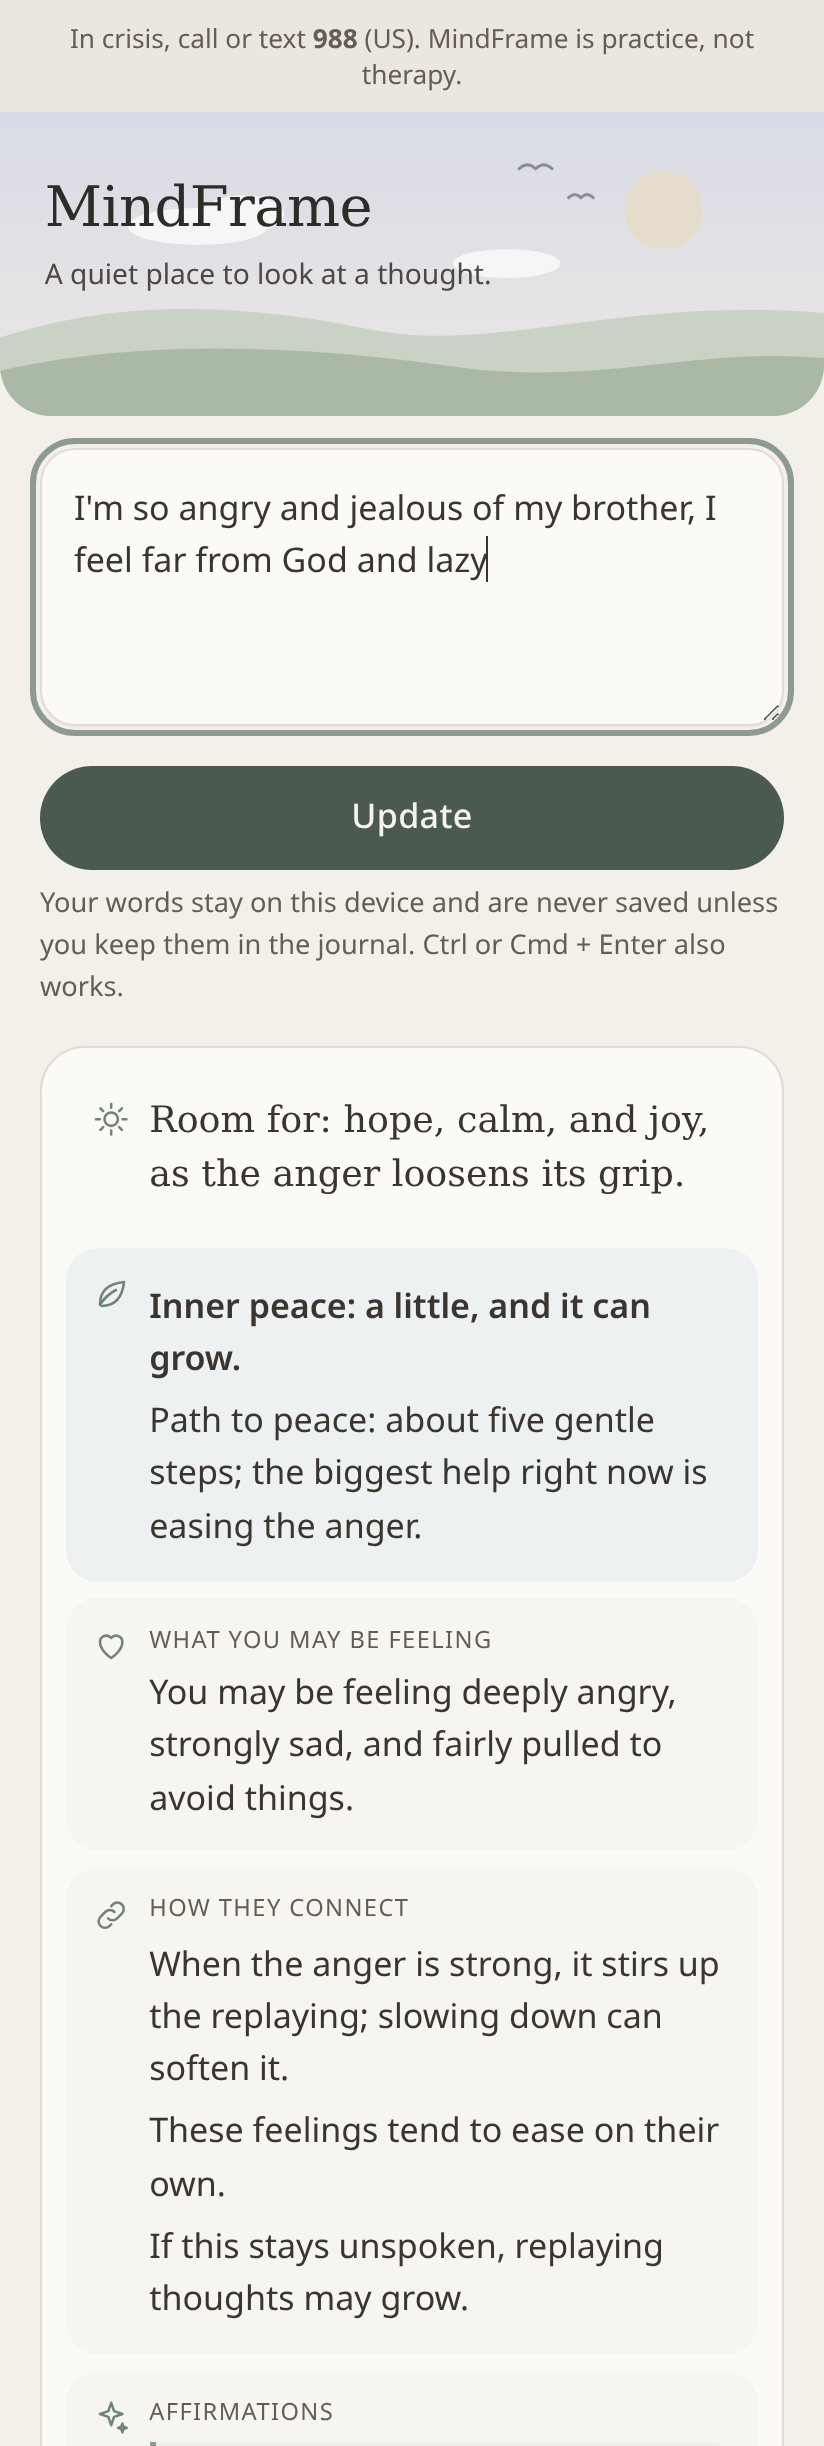
\includegraphics[width=\linewidth]{phone-top.png}
\caption{Light mode, top: input, Update, and the card's first tiles.}
\end{subfigure}\hfill
\begin{subfigure}[t]{0.31\textwidth}\centering
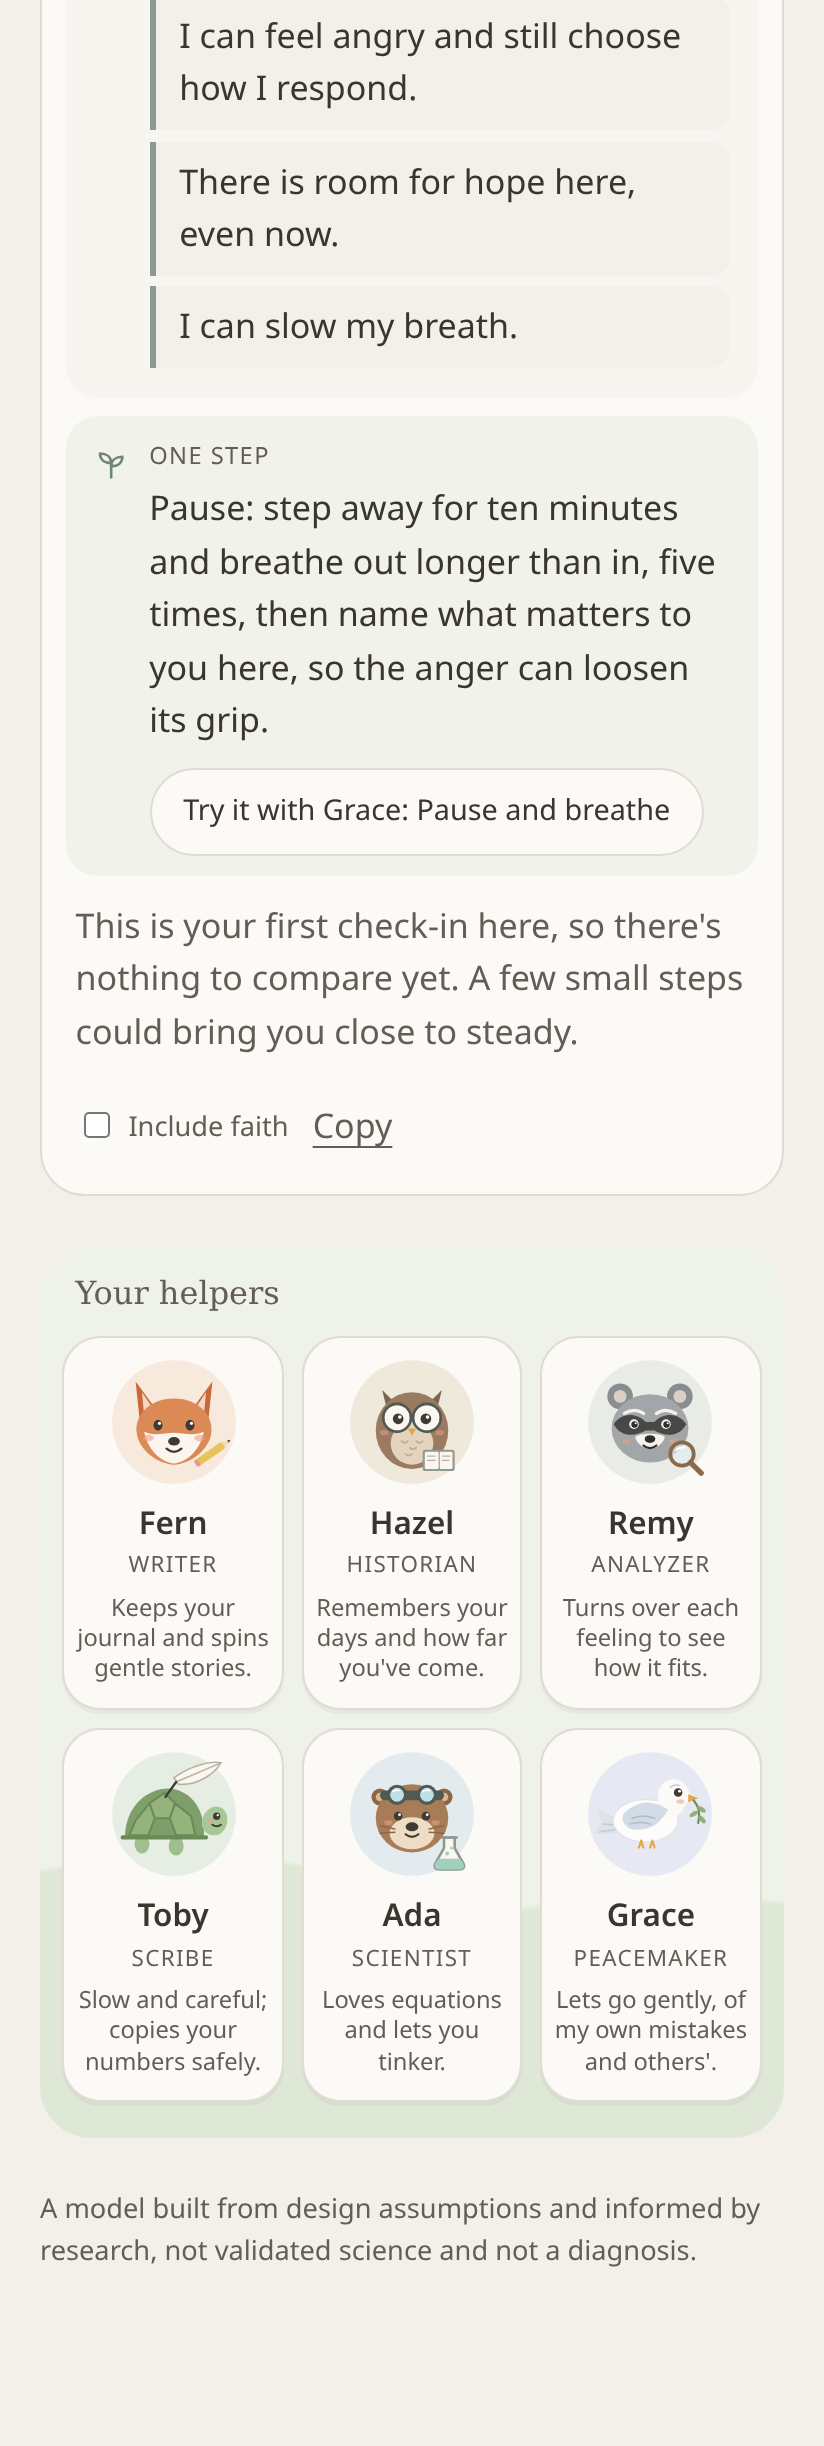
\includegraphics[width=\linewidth]{phone-bottom.png}
\caption{Light mode, continued: affirmations, the One step with ``Try it with Grace'', and the six helpers.}
\end{subfigure}\hfill
\begin{subfigure}[t]{0.31\textwidth}\centering
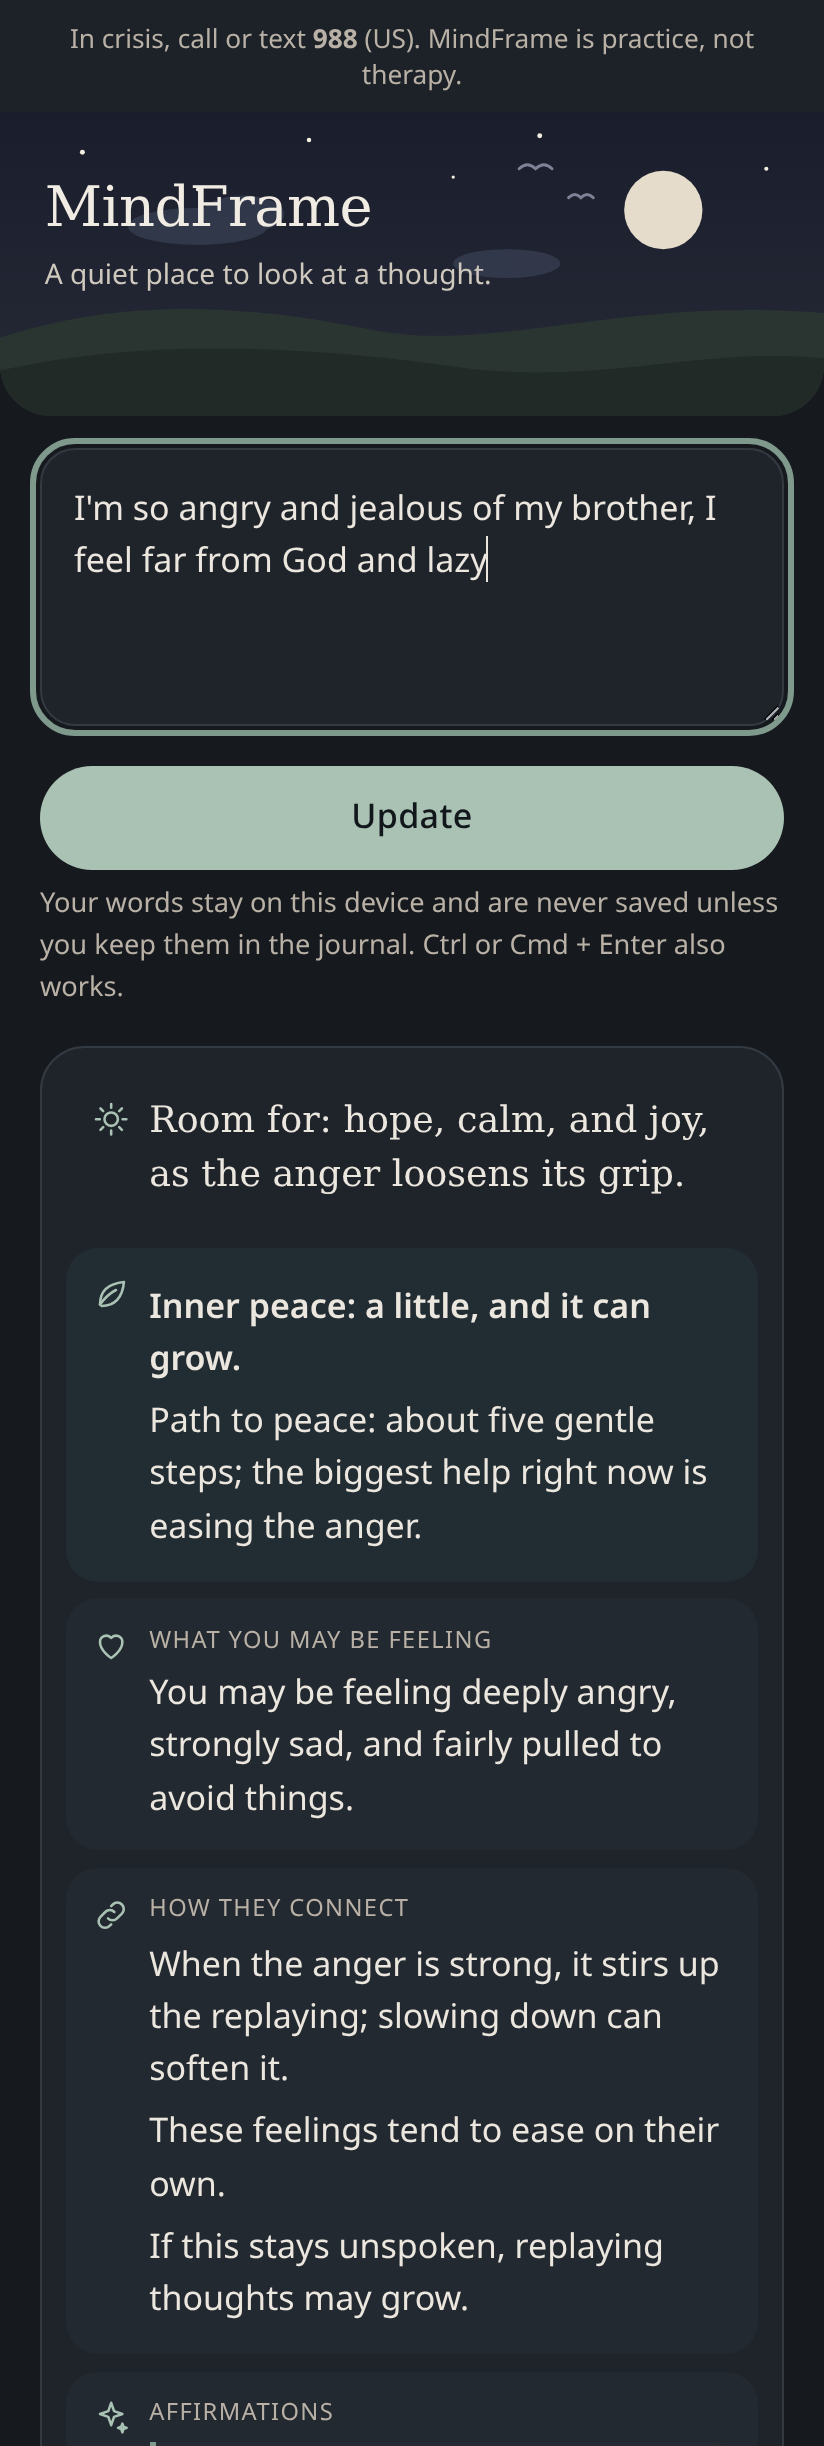
\includegraphics[width=\linewidth]{dark-top.png}
\caption{Dark mode: night sky with moon and stars; same reading.}
\end{subfigure}
\caption{The single screen on a phone, after Update, for the input ``I'm so angry and jealous of my brother, I feel far from God and lazy.'' The card shows words only. Screenshots from the build (\texttt{mf-push16-phone.png}, \texttt{mf-push16-phone-dark.png}); the light-mode capture is split into two halves.}
\label{fig:phone}
\end{figure}

\begin{figure}[tb]
\centering
\begin{subfigure}[t]{0.44\textwidth}\centering
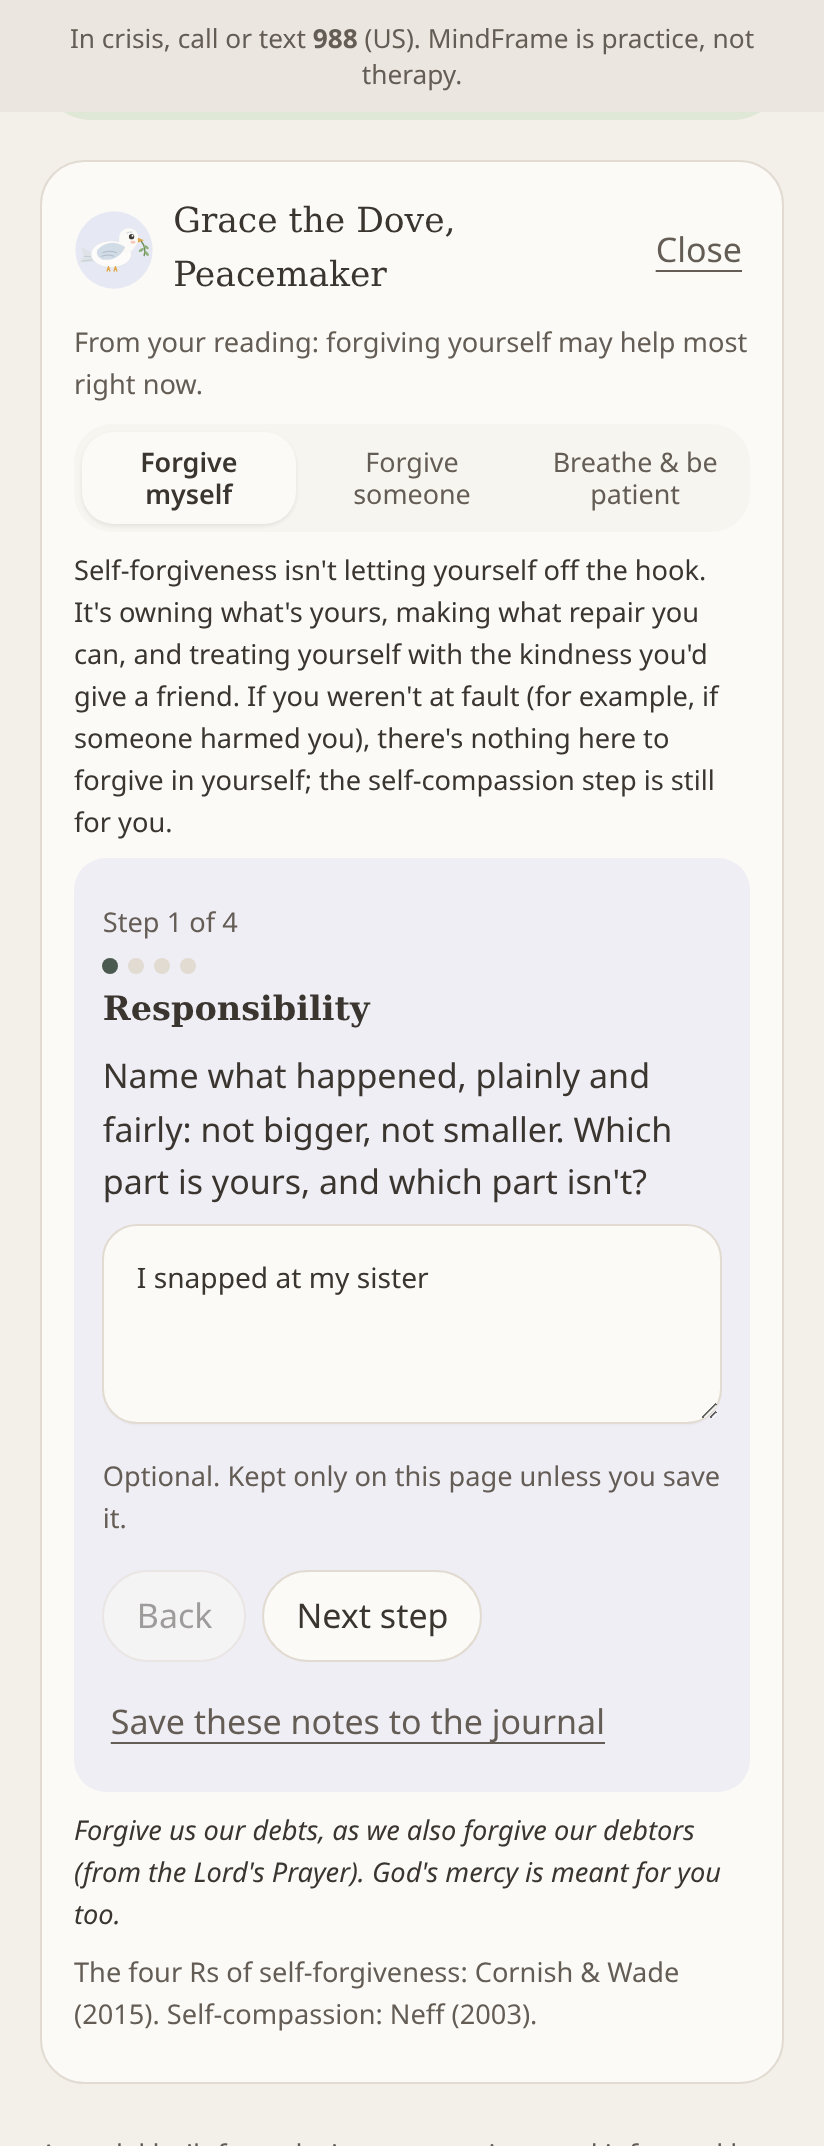
\includegraphics[height=0.5\textheight,keepaspectratio]{mf-push16-grace.png}
\caption{Grace's panel, \emph{Forgive myself}, step 1 (Responsibility), with an optional note kept only on the page. The faith line is shown because Include faith is on.}
\end{subfigure}\hfill
\begin{subfigure}[t]{0.44\textwidth}\centering
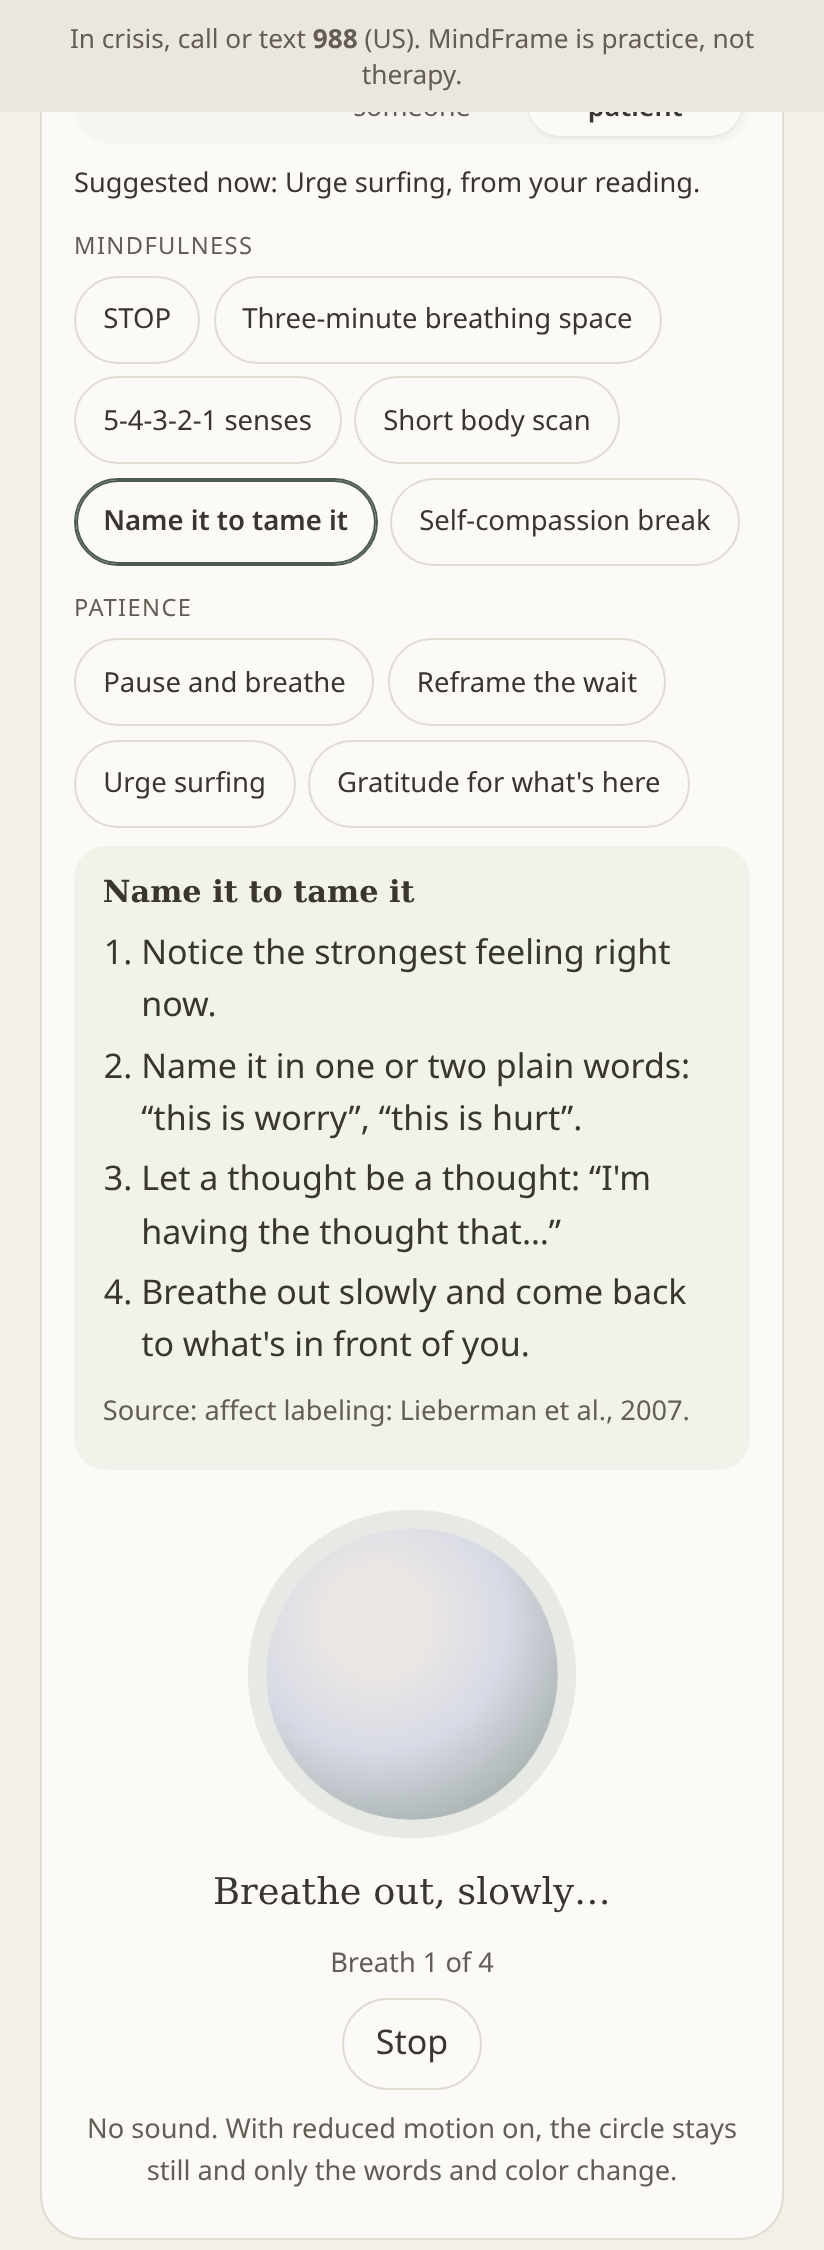
\includegraphics[height=0.5\textheight,keepaspectratio]{mf-push16-breath.png}
\caption{\emph{Breathe \& be patient}: the ten practices, the selected practice's steps and source, and the breathing circle (exhale phase).}
\end{subfigure}
\caption{Grace the Dove, Peacemaker (screenshots \texttt{mf-push16-grace.png}, \texttt{mf-push16-breath.png}).}
\label{fig:grace}
\end{figure}

%% ---------------- 11 Privacy & safety ----------------
\section{Privacy and Safety}
\label{sec:privacy}
\paragraph{Local only.} Everything stays in the browser's \texttt{localStorage}: the numbers, the faith setting, and the journal, which holds explicit saves only. The thought typed in the box is not stored unless the person saves it to the journal. Grace's note boxes are never stored unless saved. Start over clears the numbers, and Clear journal clears the journal. The \texttt{.mf} export holds numbers and labels only, never words.

\paragraph{No network calls.} The app's code makes no requests to any server. The only \texttt{fetch} is in the service worker, which serves and caches the app's own same-origin files so the page works offline (cache v17 adds the forgiveness and practice modules and the dove picture).

\paragraph{Optional public-AI comfort story.} In Fern's panel, one optional button builds a prompt for a short comfort story. The prompt is built from the \emph{words-level analysis} only: the card's composed sentences, a compact numbers summary (movers with bands, $d\to d_{\mathrm{next}}$, conflicts, $g$, $P$ with its band, $n^\star$ and the lever, the forgiveness scores and path, the chosen practice and its source), and the request. It never contains the typed text. Every line is composed from numbers, and a second guard drops any line that repeats four or more consecutive words of the input. The prompt is shown in an editable box with the note ``Only this text will be shared.'' before anything leaves the device. \emph{Open in Grok} or \emph{Open in ChatGPT} opens a new tab with the prompt in the URL and also copies it, and \emph{Copy prompt} only copies. Grok may send the prompt as soon as it opens. The button is disabled in a crisis.

\paragraph{Crisis input.} When crisis wording is detected in the input, or in any Grace note box, the master function returns only $\{\textit{crisis}\}$. The app shows only a support box (call or text 988 in the US, or call 911) and computes or saves nothing else: no peace score, no forgiveness reading, no sky colour. A banner on every screen says that MindFrame is practice, not therapy.

%% ---------------- 12 Faith ----------------
\section{The Optional Faith Toggle}
\label{sec:faith}
An \emph{Include faith} checkbox, off by default and stored locally, changes wording only and never the numbers. With it on, the card adds one affirmation and a peace verse (``May the peace of God, which surpasses all understanding, guard your heart and mind'', from Philippians). The forgiveness tiles add a line from the Lord's Prayer (self) or from Colossians (others), and Grace's panel adds Luke 23:34, ``Father, forgive them''. The practices add ``Be still, and know that I am God'' (Psalms) for mindfulness and ``Love is patient'' (1 Corinthians) for patience. A unit test checks that turning faith on changes nothing else.

%% ---------------- 13 Testing ----------------
\section{Implementation and Testing}
\label{sec:testing}
MindFrame is plain JavaScript in one shared namespace (\texttt{MF}). The model lives in \texttt{js/core} (signals, grounding, movers, reality, peace, master, words) and contains no page code. Each feature lives in its own file under \texttt{js/features}. Every file starts with a header comment, and every function has a JSDoc. Feature hooks register through \texttt{addWordHook} (nudges on existing movers) and \texttt{addPass} (fields added to master's output), so \texttt{master()} remains the one computation. The passes never change $e$, $e^{+}$, or $P$.

\paragraph{Unit tests.} There are 220 Node unit tests in ten files. For this paper we re-ran them on the build, and all passed: model 44, grounding 32, openings 31, stories 24, games 18, peace 16, reality 16, Grace 16, features 14, and practices 9. They cover the contraction and rounded-fixed-point checks above, $n^\star$ against simulation, the lever against brute force, the no-digits rule on every card line, the safety line on every forgiveness tile for others, negation handling, crisis behaviour (only \texttt{\{crisis: true\}}), the comfort prompt never containing the typed text, determinism, and faith wording changing nothing else.

\paragraph{Browser checks.} The build notes report 50 end-to-end browser checks, up from 37, on the one-screen flow, Grace's tabs, the breathing circle, dark mode, and contrast. We did not re-run them for this paper.

%% ---------------- 14 Limitations ----------------
\section{Limitations}
\label{sec:limits}
\begin{itemize}
\item \textbf{Not validated in people.} No user study, clinical trial, or measurement study has been done. Nothing here shows that MindFrame improves mood, peace, patience, or forgiveness. The cited research supports the \emph{ingredients} (for example, forgiveness interventions in \citealp{wade2014}), not this app.
\item \textbf{Keyword-based detection.} Feelings, conflicts, grandiosity, the Four Horsemen, and forgiveness cues come from stems, phrases, and regular expressions with simple negation rules. They will miss sarcasm, context, other languages, and unusual phrasing, and they can misfire. Crisis detection is also pattern-based and can fail in both directions, so it is a safety net, not a guarantee.
\item \textbf{Design-chosen weights.} $W$, the home values, every threshold ($0.3$, $0.6$, $0.25$, $P^\star=0.8$, $\theta_F=0.35$, $c_{\mathrm{wait}}\ge0.3$), the hook nudges, the release vectors, $d_0$, $\gamma$, and $\delta$ are design choices, not estimates.
\item \textbf{The proof is about the model.} Theorem~\ref{thm:contract} shows the model's arithmetic heads toward a home the designer chose. It says nothing about real emotions. The rounded iteration that the app actually runs is only tested.
\item \textbf{Forgiveness is complex.} A short guided path cannot capture forgiveness therapy, and in some situations, such as ongoing abuse, safety comes before any forgiveness work. The app states this but cannot assess it.
\item \textbf{Faith wording} reflects one tradition and is optional.
\end{itemize}

%% ---------------- 15 Future work ----------------
\section{Future Work}
\label{sec:future}
The most important next step is a small, ethically reviewed user study. It could be a within-person pilot that uses validated scales chosen in advance, for example measures of forgiveness, self-compassion, rumination, and peace of mind (the construct of \citealp{lee2013}), together with usability and safety reports. Other steps are: comparing the keyword detectors with human-labelled text and reporting their errors; a sensitivity analysis of the design weights and thresholds; a proof, or a counterexample, for termination of the rounded iteration and its bound $0.005/a$; translations and accessibility reviews with screen-reader users; and a clinical review of the crisis wording. Any study result would be reported as found, including null results.

%% ---------------- 16 Conclusion ----------------
\section{Conclusion}
MindFrame shows that a reflection tool can be small, private, and transparent at once. It uses one function over nine movers, a composer that speaks in words, and derived readings for conflict, certainty, relationship patterns, peace, forgiveness, and patience. The convergence result is a modest piece of honesty about the math: the exact map provably heads home under clear conditions, and the rounded app is tested to do so. Whether any of this helps people is an open question for future study. MindFrame is a model built from design assumptions and informed by research, not validated science and not a diagnosis.

%% ---------------- Credits and References ----------------
\section*{Credits and References}
\addcontentsline{toc}{section}{Credits and References}
\noindent\emph{With gratitude to every researcher, clinician, translator and writer listed here, whose careful work MindFrame stands on. All credit and glory to God.}

\noindent\small Every source used across MindFrame (the app, its README and its papers) was checked in October 2026. Journal articles were checked against Crossref (title, authors, year, volume, pages, DOI); books against Open Library or publisher and library catalogs; reports, preprints, archives and web articles at their source. 111 are verified; 2 are flagged and marked below. Films are credited to their studios and filmmakers and songs to their artists and songwriters; MindFrame only names them and quotes no lyrics. The works cited in this paper follow under \emph{Works cited}.

\begin{multicols}{2}
\footnotesize
\paragraph{Emotion, cognition and CBT}
\begin{itemize}[leftmargin=1em,itemsep=0pt,topsep=1pt,parsep=0pt]
\item Beck, A. T. (1976). Cognitive therapy and the emotional disorders. New York: International Universities Press.
\item Beck, A. T., Rush, A. J., Shaw, B. F., \& Emery, G. (1979). Cognitive Therapy of Depression. New York: Guilford Press.
\item Beck, J. S. (2011). Cognitive Behavior Therapy: Basics and Beyond (2nd ed.). New York: Guilford Press.
\item Beck, A. T., Steer, R. A., Kovacs, M., \& Garrison, B. (1985). Hopelessness and eventual suicide: A 10-year prospective study of patients hospitalized with suicidal ideation. American Journal of Psychiatry, 142, 559--563. \url{https://doi.org/10.1176/ajp.142.5.559}
\item Burns, D. D. (1980). Feeling good: The new mood therapy. New York: William Morrow.
\item Gross, J. J. (1998). The emerging field of emotion regulation: An integrative review. Review of General Psychology, 2(3), 271--299. \url{https://doi.org/10.1037/1089-2680.2.3.271}
\item Aldao, A., Nolen-Hoeksema, S., \& Schweizer, S. (2010). Emotion-regulation strategies across psychopathology: A meta-analytic review. Clinical Psychology Review, 30(2), 217--237. \url{https://doi.org/10.1016/j.cpr.2009.11.004}
\item Barlow, D. H., Allen, L. B., \& Choate, M. L. (2004). Toward a unified treatment for emotional disorders. Behavior Therapy, 35(2), 205--230. \url{https://doi.org/10.1016/s0005-7894(04)80036-4}
\item Nolen-Hoeksema, S., Wisco, B. E., \& Lyubomirsky, S. (2008). Rethinking rumination. Perspectives on Psychological Science, 3(5), 400--424. \url{https://doi.org/10.1111/j.1745-6924.2008.00088.x}
\item Al-Mosaiwi, M., \& Johnstone, T. (2018). In an absolute state: Elevated use of absolutist words is a marker specific to anxiety, depression, and suicidal ideation. Clinical Psychological Science, 6(4), 529--542. \url{https://doi.org/10.1177/2167702617747074}
\item Kim, S., Thibodeau, R., \& Jorgensen, R. S. (2011). Shame, guilt, and depressive symptoms: A meta-analytic review. Psychological Bulletin, 137(1), 68--96. \url{https://doi.org/10.1037/a0021466}
\item Hofmann, S. G., Asnaani, A., Vonk, I. J. J., Sawyer, A. T., \& Fang, A. (2012). The efficacy of cognitive behavioral therapy: A review of meta-analyses. Cognitive Therapy and Research, 36(5), 427--440. \url{https://doi.org/10.1007/s10608-012-9476-1}
\item Lieberman, M. D., Eisenberger, N. I., Crockett, M. J., Tom, S. M., Pfeifer, J. H., \& Way, B. M. (2007). Putting feelings into words: Affect labeling disrupts amygdala activity in response to affective stimuli. Psychological Science, 18(5), 421--428. \url{https://doi.org/10.1111/j.1467-9280.2007.01916.x}
\item Snyder, C. R. (2002). Hope theory: Rainbows in the mind. Psychological Inquiry, 13(4), 249--275. \url{https://doi.org/10.1207/s15327965pli1304_01}
\item Wolpe, J. (1969). The Practice of Behavior Therapy. New York: Pergamon Press.
\item Rachman, S., \& de Silva, P. (1978). Abnormal and normal obsessions. Behaviour Research and Therapy, 16(4), 233--248. \url{https://doi.org/10.1016/0005-7967(78)90022-0}
\item Holmes, E. A., \& Mathews, A. (2010). Mental imagery in emotion and emotional disorders. Clinical Psychology Review, 30(3), 349--362. \url{https://doi.org/10.1016/j.cpr.2010.01.001}
\item Wegner, D. M., Schneider, D. J., Carter, S. R., \& White, T. L. (1987). Paradoxical effects of thought suppression. Journal of Personality and Social Psychology, 53(1), 5--13. \url{https://doi.org/10.1037/0022-3514.53.1.5}
\item Borkovec, T. D., Wilkinson, L., Folensbee, R., \& Lerman, C. (1983). Stimulus control applications to the treatment of worry. Behaviour Research and Therapy, 21(3), 247--251. \url{https://doi.org/10.1016/0005-7967(83)90206-1}
\item McGowan, S. K., \& Behar, E. (2013). A preliminary investigation of stimulus control training for worry: Effects on anxiety and insomnia. Behavior Modification, 37(1), 90--112. \url{https://doi.org/10.1177/0145445512455661}
\item King, L. A. (2001). The health benefits of writing about life goals. Personality and Social Psychology Bulletin, 27(7), 798--807. \url{https://doi.org/10.1177/0146167201277003}
\item Peters, M. L., Flink, I. K., Boersma, K., \& Linton, S. J. (2010). Manipulating optimism: Can imagining a best possible self be used to increase positive future expectancies? The Journal of Positive Psychology, 5(3), 204--211. \url{https://doi.org/10.1080/17439761003790963}
\item Hershfield, H. E. (2011). Future self-continuity: How conceptions of the future self transform intertemporal choice. Annals of the New York Academy of Sciences, 1235, 30--43. \url{https://doi.org/10.1111/j.1749-6632.2011.06201.x}
\item Oettingen, G. (2014). Rethinking Positive Thinking: Inside the New Science of Motivation. New York: Current.
\item American Psychiatric Association. (2013). Diagnostic and Statistical Manual of Mental Disorders (5th ed.). Arlington, VA: APA. \url{https://doi.org/10.1176/appi.books.9780890425596}
\item Kroenke, K., Strine, T. W., Spitzer, R. L., Williams, J. B. W., Berry, J. T., \& Mokdad, A. H. (2009). The PHQ-8 as a measure of current depression in the general population. Journal of Affective Disorders, 114(1--3), 163--173. \url{https://doi.org/10.1016/j.jad.2008.06.026}
\item Shiffman, S., Stone, A. A., \& Hufford, M. R. (2008). Ecological momentary assessment. Annual Review of Clinical Psychology, 4, 1--32. \url{https://doi.org/10.1146/annurev.clinpsy.3.022806.091415}
\item Dawes, R. M. (1979). The robust beauty of improper linear models in decision making. American Psychologist, 34(7), 571--582. \url{https://doi.org/10.1037/0003-066x.34.7.571}
\item Kravitz, R. L., Duan, N., \& the DEcIDE Methods Center N-of-1 Guidance Panel (Eds.). (2014). Design and Implementation of N-of-1 Trials: A User's Guide. Rockville, MD: Agency for Healthcare Research and Quality.
\item Fitzpatrick, K. K., Darcy, A., \& Vierhile, M. (2017). Delivering cognitive behavior therapy to young adults with symptoms of depression and anxiety using a fully automated conversational agent (Woebot): A randomized controlled trial. JMIR Mental Health, 4(2), e19. \url{https://doi.org/10.2196/mental.7785}
\item Cohen, G. L., \& Sherman, D. K. (2014). The psychology of change: Self-affirmation and social psychological intervention. Annual Review of Psychology, 65, 333--371. \url{https://doi.org/10.1146/annurev-psych-010213-115137}
\end{itemize}
\paragraph{DBT, ACT, mindfulness and compassion}
\begin{itemize}[leftmargin=1em,itemsep=0pt,topsep=1pt,parsep=0pt]
\item Linehan, M. M. (1993). Cognitive-Behavioral Treatment of Borderline Personality Disorder. New York: Guilford Press.
\item Linehan, M. M. (2015). DBT skills training manual (2nd ed.). New York: Guilford Press. (TIP skills: Temperature).
\item Neacsiu, A. D., Rizvi, S. L., \& Linehan, M. M. (2010). Dialectical behavior therapy skills use as a mediator and outcome of treatment for borderline personality disorder. Behaviour Research and Therapy, 48(9), 832--839. \url{https://doi.org/10.1016/j.brat.2010.05.017}
\item Neacsiu, A. D., Rizvi, S. L., Vitaliano, P. P., Lynch, T. R., \& Linehan, M. M. (2010). The Dialectical Behavior Therapy Ways of Coping Checklist: Development and psychometric properties. Journal of Clinical Psychology, 66(6), 563--582. \url{https://doi.org/10.1002/jclp.20685}
\item Hayes, S. C., Luoma, J. B., Bond, F. W., Masuda, A., \& Lillis, J. (2006). Acceptance and commitment therapy: Model, processes and outcomes. Behaviour Research and Therapy, 44(1), 1--25. \url{https://doi.org/10.1016/j.brat.2005.06.006}
\item Hayes, S. C., Strosahl, K. D., \& Wilson, K. G. (2012). Acceptance and Commitment Therapy: The Process and Practice of Mindful Change (2nd ed.). New York: Guilford Press.
\item Masuda, A., Hayes, S. C., Sackett, C. F., \& Twohig, M. P. (2004). Cognitive defusion and self-relevant negative thoughts: Examining the impact of a ninety year old technique. Behaviour Research and Therapy, 42(4), 477--485. \url{https://doi.org/10.1016/j.brat.2003.10.008}
\item Bond, F. W., et al. (2011). Preliminary psychometric properties of the Acceptance and Action Questionnaire--II. Behavior Therapy, 42(4), 676--688. \url{https://doi.org/10.1016/j.beth.2011.03.007}
\item Gillanders, D. T., et al. (2014). The development and initial validation of the Cognitive Fusion Questionnaire. Behavior Therapy, 45(1), 83--101. \url{https://doi.org/10.1016/j.beth.2013.09.001}
\item Kabat-Zinn, J. (1990). Full catastrophe living. New York: Delacorte.
\item Kabat-Zinn, J. (2003). Mindfulness-based interventions in context: Past, present, and future. Clinical Psychology: Science and Practice, 10(2), 144--156. \url{https://doi.org/10.1093/clipsy.bpg016}
\item Segal, Z. V., Williams, J. M. G., \& Teasdale, J. D. (2013). Mindfulness-based cognitive therapy for depression (2nd ed.). New York: Guilford Press.
\item Stahl, B., \& Goldstein, E. (2010). A mindfulness-based stress reduction workbook. Oakland, CA: New Harbinger.
\item Desbordes, G., Gard, T., Hoge, E. A., Hölzel, B. K., Kerr, C., Lazar, S. W., Olendzki, A., \& Vago, D. R. (2015). Moving beyond mindfulness: Defining equanimity as an outcome measure in meditation and contemplative research. Mindfulness, 6(2), 356--372. \url{https://doi.org/10.1007/s12671-013-0269-8}
\item Neff, K. D. (2003). Self-compassion: An alternative conceptualization of a healthy attitude toward oneself. Self and Identity, 2(2), 85--101. \url{https://doi.org/10.1080/15298860309032}
\item Gilbert, P. (2009). Introducing compassion-focused therapy. Advances in Psychiatric Treatment, 15(3), 199--208. \url{https://doi.org/10.1192/apt.bp.107.005264}
\item Gilbert, P., \& Procter, S. (2006). Compassionate mind training for people with high shame and self-criticism: Overview and pilot study of a group therapy approach. Clinical Psychology \& Psychotherapy, 13(6), 353--379. \url{https://doi.org/10.1002/cpp.507}
\item Hofmann, S. G., Grossman, P., \& Hinton, D. E. (2011). Loving-kindness and compassion meditation: Potential for psychological interventions. Clinical Psychology Review, 31(7), 1126--1132. \url{https://doi.org/10.1016/j.cpr.2011.07.003}
\item Bowen, S., \& Marlatt, A. (2009). Surfing the urge: Brief mindfulness-based intervention for college student smokers. Psychology of Addictive Behaviors, 23(4), 666--671. \url{https://doi.org/10.1037/a0017127}
\item Miller, W. R., \& Rollnick, S. (2013). Motivational interviewing: Helping people change (3rd ed.). New York: Guilford Press.
\item Zaccaro, A., et al. (2018). How breath-control can change your life: A systematic review on psycho-physiological correlates of slow breathing. Frontiers in Human Neuroscience, 12, 353. \url{https://doi.org/10.3389/fnhum.2018.00353}
\end{itemize}
\paragraph{Forgiveness, virtue, gratitude and peace}
\begin{itemize}[leftmargin=1em,itemsep=0pt,topsep=1pt,parsep=0pt]
\item Cornish, M. A., \& Wade, N. G. (2015). A therapeutic model of self-forgiveness with intervention strategies for counselors. Journal of Counseling \& Development, 93(1), 96--104. \url{https://doi.org/10.1002/j.1556-6676.2015.00185.x}
\item Worthington, E. L., Jr. (2006). Forgiveness and reconciliation: Theory and application. New York: Routledge.
\item Wade, N. G., Hoyt, W. T., Kidwell, J. E. M., \& Worthington, E. L., Jr. (2014). Efficacy of psychotherapeutic interventions to promote forgiveness: A meta-analysis. Journal of Consulting and Clinical Psychology, 82(1), 154--170. \url{https://doi.org/10.1037/a0035268}
\item Enright, R. D., \& Fitzgibbons, R. P. (2015). Forgiveness therapy: An empirical guide for resolving anger and restoring hope. Washington, DC: APA. \url{https://doi.org/10.1037/14526-000}
\item McCullough, M. E., Bono, G., \& Root, L. M. (2007). Rumination, emotion, and forgiveness: Three longitudinal studies. Journal of Personality and Social Psychology, 92(3), 490--505. \url{https://doi.org/10.1037/0022-3514.92.3.490}
\item Emmons, R. A., \& McCullough, M. E. (2003). Counting blessings versus burdens: An experimental investigation of gratitude and subjective well-being in daily life. Journal of Personality and Social Psychology, 84(2), 377--389. \url{https://doi.org/10.1037/0022-3514.84.2.377}
\item Schnitker, S. A. (2012). An examination of patience and well-being. The Journal of Positive Psychology, 7(4), 263--280. \url{https://doi.org/10.1080/17439760.2012.697185}
\item Tangney, J. P. (2000). Humility: Theoretical perspectives, empirical findings and directions for future research. Journal of Social and Clinical Psychology, 19(1), 70--82. \url{https://doi.org/10.1521/jscp.2000.19.1.70}
\item Lee, Y.-C., Lin, Y.-C., Huang, C.-L., \& Fredrickson, B. L. (2013). The construct and measurement of peace of mind. Journal of Happiness Studies, 14(2), 571--590. \url{https://doi.org/10.1007/s10902-012-9343-5}
\item Davis, M. H. (1983). Measuring individual differences in empathy: Evidence for a multidimensional approach. Journal of Personality and Social Psychology, 44(1), 113--126. \url{https://doi.org/10.1037/0022-3514.44.1.113}
\item Speed, B. C., Goldstein, B. L., \& Goldfried, M. R. (2018). Assertiveness training: A forgotten evidence-based treatment. Clinical Psychology: Science and Practice, 25(1), e12216. \url{https://doi.org/10.1111/cpsp.12216}
\end{itemize}
\paragraph{Relationships and belonging}
\begin{itemize}[leftmargin=1em,itemsep=0pt,topsep=1pt,parsep=0pt]
\item Gottman, J. M. (1994). What predicts divorce? The relationship between marital processes and marital outcomes. Hillsdale, NJ: Erlbaum.
\item Gottman, J. M., \& Levenson, R. W. (1992). Marital processes predictive of later dissolution: Behavior, physiology, and health. Journal of Personality and Social Psychology, 63(2), 221--233. \url{https://doi.org/10.1037/0022-3514.63.2.221}
\item Gottman, J. M., \& Levenson, R. W. (2000). The timing of divorce: Predicting when a couple will divorce over a 14-year period. Journal of Marriage and Family, 62(3), 737--745. \url{https://doi.org/10.1111/j.1741-3737.2000.00737.x}
\item Heyman, R. E., \& Slep, A. M. S. (2001). The hazards of predicting divorce without crossvalidation. Journal of Marriage and Family, 63(2), 473--479. \url{https://doi.org/10.1111/j.1741-3737.2001.00473.x}
\item Holt-Lunstad, J., Smith, T. B., \& Layton, J. B. (2010). Social relationships and mortality risk: A meta-analytic review. PLoS Medicine, 7(7), e1000316. \url{https://doi.org/10.1371/journal.pmed.1000316}
\item Baumeister, R. F., \& Leary, M. R. (1995). The need to belong: Desire for interpersonal attachments as a fundamental human motivation. Psychological Bulletin, 117(3), 497--529. \url{https://doi.org/10.1037/0033-2909.117.3.497}
\item Meng, X., Chen, Y., Wang, X., Yuan, J., \& Yu, D. (2024). The relationship between school connectedness and depression: A three-level meta-analytic review. Advances in Psychological Science, 32(2), 246--263. (In Chinese with English abstract.). \url{https://doi.org/10.3724/sp.j.1042.2024.00246}
\end{itemize}
\paragraph{Body, writing and activity}
\begin{itemize}[leftmargin=1em,itemsep=0pt,topsep=1pt,parsep=0pt]
\item Jacobson, E. (1938). Progressive relaxation (2nd ed.). Chicago: University of Chicago Press.
\item McCallie, M. S., Blum, C. M., \& Hood, C. J. (2006). Progressive muscle relaxation. Journal of Human Behavior in the Social Environment, 13(3), 51--66. \url{https://doi.org/10.1300/j137v13n03_04}
\item Pennebaker, J. W., \& Beall, S. K. (1986). Confronting a traumatic event: Toward an understanding of inhibition and disease. Journal of Abnormal Psychology, 95(3), 274--281. \url{https://doi.org/10.1037/0021-843x.95.3.274}
\item Frattaroli, J. (2006). Experimental disclosure and its moderators: A meta-analysis. Psychological Bulletin, 132(6), 823--865. (146 studies; a small average effect, r $\approx$ .08). \url{https://doi.org/10.1037/0033-2909.132.6.823}
\item Ekkekakis, P., Hall, E. E., VanLanduyt, L. M., \& Petruzzello, S. J. (2000). Walking in (affective) circles: Can short walks enhance affect? Journal of Behavioral Medicine, 23(3), 245--275. \url{https://doi.org/10.1023/a:1005558025163}
\item Rebar, A. L., Stanton, R., Geard, D., Short, C., Duncan, M. J., \& Vandelanotte, C. (2015). A meta-meta-analysis of the effect of physical activity on depression and anxiety in non-clinical adult populations. Health Psychology Review, 9(3), 366--378. \url{https://doi.org/10.1080/17437199.2015.1022901}
\end{itemize}
\paragraph{Inner speech, language and design}
\begin{itemize}[leftmargin=1em,itemsep=0pt,topsep=1pt,parsep=0pt]
\item Alderson-Day, B., \& Fernyhough, C. (2015). Inner speech: Development, cognitive functions, phenomenology, and neurobiology. Psychological Bulletin, 141(5), 931--965. \url{https://doi.org/10.1037/bul0000021}
\item Fernyhough, C. (2016). The Voices Within: The History and Science of How We Talk to Ourselves. New York: Basic Books.
\item Kross, E., Bruehlman-Senecal, E., Park, J., et al. (2014). Self-talk as a regulatory mechanism: How you do it matters. Journal of Personality and Social Psychology, 106(2), 304--324. \url{https://doi.org/10.1037/a0035173}
\item Vygotsky, L. S. (1986). Thought and Language (A. Kozulin, Ed. \& Trans.). Cambridge, MA: MIT Press. (Original work published 1934.).
\item Whorf, B. L. (1956). Language, Thought, and Reality (J. B. Carroll, Ed.). Cambridge, MA: MIT Press.
\item Boroditsky, L. (2001). Does language shape thought? Mandarin and English speakers' conceptions of time. Cognitive Psychology, 43(1), 1--22. \url{https://doi.org/10.1006/cogp.2001.0748}
\item Cowan, N. (2001). The magical number 4 in short-term memory: A reconsideration of mental storage capacity. Behavioral and Brain Sciences, 24(1), 87--114. \url{https://doi.org/10.1017/s0140525x01003922}
\item Miller, G. A. (1956). The magical number seven, plus or minus two: Some limits on our capacity for processing information. Psychological Review, 63(2), 81--97. \url{https://doi.org/10.1037/h0043158}
\item Sweller, J. (1988). Cognitive load during problem solving: Effects on learning. Cognitive Science, 12(2), 257--285. \url{https://doi.org/10.1207/s15516709cog1202_4}
\item Nielsen, J. (2006). Progressive disclosure. Nielsen Norman Group article, nngroup.com.
\item Weizenbaum, J. (1966). ELIZA---A computer program for the study of natural language communication between man and machine. Communications of the ACM, 9(1), 36--45. \url{https://doi.org/10.1145/365153.365168}
\item Bommasani, R., et al. (2021). On the opportunities and risks of foundation models. arXiv preprint arXiv:2108.07258. \url{https://doi.org/10.48550/arXiv.2108.07258}
\end{itemize}
\paragraph{Media}
\begin{itemize}[leftmargin=1em,itemsep=0pt,topsep=1pt,parsep=0pt]
\item Zillmann, D. (1988). Mood management through communication choices. American Behavioral Scientist, 31(3), 327--340. \url{https://doi.org/10.1177/000276488031003005}
\end{itemize}
\paragraph{Mathematics}
\begin{itemize}[leftmargin=1em,itemsep=0pt,topsep=1pt,parsep=0pt]
\item Langlands, R. P. (1967). Letter to André Weil. (Available via the Institute for Advanced Study's Langlands archive.).
\item Gelbart, S. (1984). An elementary introduction to the Langlands program. Bulletin of the American Mathematical Society, 10(2), 177--219. \url{https://doi.org/10.1090/s0273-0979-1984-15237-6}
\item Wiles, A. (1995). Modular elliptic curves and Fermat's Last Theorem. Annals of Mathematics, 141(3), 443--551. \url{https://doi.org/10.2307/2118559}
\item Frenkel, E. (2013). Love and Math: The Heart of Hidden Reality. New York: Basic Books.
\end{itemize}
\paragraph{Philosophy and spiritual writers}
\begin{itemize}[leftmargin=1em,itemsep=0pt,topsep=1pt,parsep=0pt]
\item Frankl, V. E. (2006). Man's Search for Meaning. Boston: Beacon Press. (Original work published 1946.).
\item Robertson, D. (2010). The Philosophy of Cognitive-Behavioural Therapy (CBT): Stoic Philosophy as Rational and Cognitive Psychotherapy. London: Karnac.
\item Epictetus. (c. 125 CE). Enchiridion (Handbook). Various translations. \textit{[Flagged: Classical work (Enchiridion); existence is certain, but the paper names no edition or translator, so no full citation can be verified.]}
\item Marcus Aurelius. (c. 170--180 CE). Meditations. Various translations. \textit{[Flagged: Classical work (Meditations); existence is certain, but the paper names no edition or translator, so no full citation can be verified.]}
\item Teresa of Ávila. The interior castle (VI.10.7). In K. Kavanaugh \& O. Rodriguez (Trans.), The collected works of St. Teresa of Avila (Vol. 2). Washington, DC: ICS Publications, 1980. ("To be humble is to walk in truth.").
\end{itemize}
\paragraph{Time, dynamics, control and imagery}
\begin{itemize}[leftmargin=1em,itemsep=0pt,topsep=1pt,parsep=0pt]
\item Verduyn, P., \& Lavrijsen, S. (2015). Which emotions last longest and why: The role of event importance and rumination. Motivation and Emotion, 39(1), 119--127. \url{https://doi.org/10.1007/s11031-014-9445-y}
\item Verduyn, P., Delvaux, E., Van Coillie, H., Tuerlinckx, F., \& Van Mechelen, I. (2009). Predicting the duration of emotional experience: Two experience sampling studies. Emotion, 9(1), 83--91. \url{https://doi.org/10.1037/a0014610}
\item Kuppens, P., Allen, N. B., \& Sheeber, L. B. (2010). Emotional inertia and psychological maladjustment. Psychological Science, 21(7), 984--991. \url{https://doi.org/10.1177/0956797610372634}
\item Banach, S. (1922). Sur les opérations dans les ensembles abstraits et leur application aux équations intégrales. Fundamenta Mathematicae, 3, 133--181. \url{https://doi.org/10.4064/fm-3-1-133-181}
\item Lyapunov, A. M. (1992). The general problem of the stability of motion (A. T. Fuller, Trans.). International Journal of Control, 55(3), 531--773. (Original work published 1892). \url{https://doi.org/10.1080/00207179208934253}
\item Åström, K. J., \& Murray, R. M. (2008). Feedback Systems: An Introduction for Scientists and Engineers. Princeton, NJ: Princeton University Press. \url{https://doi.org/10.1515/9781400828739}
\item Kaplan, S. (1995). The restorative benefits of nature: Toward an integrative framework. Journal of Environmental Psychology, 15(3), 169--182. \url{https://doi.org/10.1016/0272-4944(95)90001-2}
\item Berman, M. G., Jonides, J., \& Kaplan, S. (2008). The cognitive benefits of interacting with nature. Psychological Science, 19(12), 1207--1212. \url{https://doi.org/10.1111/j.1467-9280.2008.02225.x}
\item Curry, O. S., Rowland, L. A., Van Lissa, C. J., Zlotowitz, S., McAlaney, J., \& Whitehouse, H. (2018). Happy to help? A systematic review and meta-analysis of the effects of performing acts of kindness on the well-being of the actor. Journal of Experimental Social Psychology, 76, 320--329. \url{https://doi.org/10.1016/j.jesp.2018.02.014}
\item Lewinsohn, P. M. (1974). A behavioral approach to depression. In R. J. Friedman \& M. M. Katz (Eds.), The psychology of depression: Contemporary theory and research (pp. 157--178). Washington, DC: V. H. Winston \& Sons / Wiley.
\item Martell, C. R., Addis, M. E., \& Jacobson, N. S. (2001). Depression in context: Strategies for guided action. New York: W. W. Norton.
\item Csikszentmihalyi, M. (1990). Flow: The psychology of optimal experience. New York: Harper \& Row.
\end{itemize}
\paragraph{Scripture and data}
\begin{itemize}[leftmargin=1em,itemsep=0pt,topsep=1pt,parsep=0pt]
\item World English Bible (public domain). eBible.org, eng-web\_vpl.txt (sha256 52b92dc6\ldots{}cd8c4).
\item Wikidata (CC0), Wikimedia Foundation. Film titles, years and ids in the films list.
\item The Movie Database (TMDB) API, optional and off by default. This product uses the TMDB API but is not endorsed or certified by TMDB.
\end{itemize}
\end{multicols}
\normalsize
\renewcommand{\refname}{Works cited}
%% ---------------- References ----------------
\begin{multicols}{2}
\begin{thebibliography}{99}\footnotesize
\setlength{\itemsep}{1pt}

\bibitem[Al-Mosaiwi and Johnstone(2018)]{almosaiwi2018}
Al-Mosaiwi, M., \& Johnstone, T. (2018). In an absolute state: Elevated use of absolutist words is a marker specific to anxiety, depression, and suicidal ideation. \emph{Clinical Psychological Science, 6}(4), 529--542. doi:10.1177/2167702617747074

\bibitem[Aldao et~al.(2010)]{aldao2010}
Aldao, A., Nolen-Hoeksema, S., \& Schweizer, S. (2010). Emotion-regulation strategies across psychopathology: A meta-analytic review. \emph{Clinical Psychology Review, 30}(2), 217--237.

\bibitem[Barlow et~al.(2004)]{barlow2004}
Barlow, D. H., Allen, L. B., \& Choate, M. L. (2004). Toward a unified treatment for emotional disorders. \emph{Behavior Therapy, 35}(2), 205--230. doi:10.1016/S0005-7894(04)80036-4

\bibitem[Beck(1976)]{beck1976}
Beck, A. T. (1976). \emph{Cognitive therapy and the emotional disorders.} New York: International Universities Press.

\bibitem[Beck et~al.(1985)]{beck1985}
Beck, A. T., Steer, R. A., Kovacs, M., \& Garrison, B. (1985). Hopelessness and eventual suicide: A 10-year prospective study of patients hospitalized with suicidal ideation. \emph{American Journal of Psychiatry, 142}, 559--563.

\bibitem[Bond et~al.(2011)]{bond2011}
Bond, F. W., et al. (2011). Preliminary psychometric properties of the Acceptance and Action Questionnaire--II. \emph{Behavior Therapy, 42}(4), 676--688.

\bibitem[Bowen and Marlatt(2009)]{bowen2009}
Bowen, S., \& Marlatt, A. (2009). Surfing the urge: Brief mindfulness-based intervention for college student smokers. \emph{Psychology of Addictive Behaviors, 23}(4), 666--671. doi:10.1037/a0017127

\bibitem[Burns(1980)]{burns1980}
Burns, D. D. (1980). \emph{Feeling good: The new mood therapy.} New York: William Morrow.

\bibitem[Cornish and Wade(2015)]{cornish2015}
Cornish, M. A., \& Wade, N. G. (2015). A therapeutic model of self-forgiveness with intervention strategies for counselors. \emph{Journal of Counseling \& Development, 93}(1), 96--104. doi:10.1002/j.1556-6676.2015.00185.x

\bibitem[Desbordes et~al.(2015)]{desbordes2015}
Desbordes, G., Gard, T., Hoge, E. A., H\"olzel, B. K., Kerr, C., Lazar, S. W., Olendzki, A., \& Vago, D. R. (2015). Moving beyond mindfulness: Defining equanimity as an outcome measure in meditation and contemplative research. \emph{Mindfulness, 6}(2), 356--372. doi:10.1007/s12671-013-0269-8

\bibitem[Emmons and McCullough(2003)]{emmons2003}
Emmons, R. A., \& McCullough, M. E. (2003). Counting blessings versus burdens: An experimental investigation of gratitude and subjective well-being in daily life. \emph{Journal of Personality and Social Psychology, 84}(2), 377--389.

\bibitem[Enright and Fitzgibbons(2015)]{enright2015}
Enright, R. D., \& Fitzgibbons, R. P. (2015). \emph{Forgiveness therapy: An empirical guide for resolving anger and restoring hope.} Washington, DC: American Psychological Association. doi:10.1037/14526-000

\bibitem[Gillanders et~al.(2014)]{gillanders2014}
Gillanders, D. T., et al. (2014). The development and initial validation of the Cognitive Fusion Questionnaire. \emph{Behavior Therapy, 45}(1), 83--101.

\bibitem[Gottman(1994)]{gottman1994}
Gottman, J. M. (1994). \emph{What predicts divorce? The relationship between marital processes and marital outcomes.} Hillsdale, NJ: Erlbaum.

\bibitem[Gottman and Levenson(1992)]{gottman1992}
Gottman, J. M., \& Levenson, R. W. (1992). Marital processes predictive of later dissolution: Behavior, physiology, and health. \emph{Journal of Personality and Social Psychology, 63}(2), 221--233. doi:10.1037/0022-3514.63.2.221

\bibitem[Gottman and Levenson(2000)]{gottman2000}
Gottman, J. M., \& Levenson, R. W. (2000). The timing of divorce: Predicting when a couple will divorce over a 14-year period. \emph{Journal of Marriage and Family, 62}(3), 737--745.

\bibitem[Gross(1998)]{gross1998}
Gross, J. J. (1998). The emerging field of emotion regulation: An integrative review. \emph{Review of General Psychology, 2}(3), 271--299.

\bibitem[Heyman and Slep(2001)]{heyman2001}
Heyman, R. E., \& Slep, A. M. S. (2001). The hazards of predicting divorce without crossvalidation. \emph{Journal of Marriage and Family, 63}(2), 473--479. doi:10.1111/j.1741-3737.2001.00473.x

\bibitem[Holt-Lunstad et~al.(2010)]{holtlunstad2010}
Holt-Lunstad, J., Smith, T. B., \& Layton, J. B. (2010). Social relationships and mortality risk: A meta-analytic review. \emph{PLoS Medicine, 7}(7), e1000316.

\bibitem[Kabat-Zinn(1990)]{kabatzinn1990}
Kabat-Zinn, J. (1990). \emph{Full catastrophe living.} New York: Delacorte.

\bibitem[Kabat-Zinn(2003)]{kabatzinn2003}
Kabat-Zinn, J. (2003). Mindfulness-based interventions in context: Past, present, and future. \emph{Clinical Psychology: Science and Practice, 10}(2), 144--156. doi:10.1093/clipsy.bpg016

\bibitem[Kim et~al.(2011)]{kim2011}
Kim, S., Thibodeau, R., \& Jorgensen, R. S. (2011). Shame, guilt, and depressive symptoms: A meta-analytic review. \emph{Psychological Bulletin, 137}(1), 68--96. doi:10.1037/a0021466

\bibitem[Lee et~al.(2013)]{lee2013}
Lee, Y.-C., Lin, Y.-C., Huang, C.-L., \& Fredrickson, B. L. (2013). The construct and measurement of peace of mind. \emph{Journal of Happiness Studies, 14}(2), 571--590. doi:10.1007/s10902-012-9343-5

\bibitem[Lieberman et~al.(2007)]{lieberman2007}
Lieberman, M. D., Eisenberger, N. I., Crockett, M. J., Tom, S. M., Pfeifer, J. H., \& Way, B. M. (2007). Putting feelings into words: Affect labeling disrupts amygdala activity in response to affective stimuli. \emph{Psychological Science, 18}(5), 421--428.

\bibitem[McCullough et~al.(2007)]{mccullough2007}
McCullough, M. E., Bono, G., \& Root, L. M. (2007). Rumination, emotion, and forgiveness: Three longitudinal studies. \emph{Journal of Personality and Social Psychology, 92}(3), 490--505. doi:10.1037/0022-3514.92.3.490

\bibitem[Miller and Rollnick(2013)]{miller2013}
Miller, W. R., \& Rollnick, S. (2013). \emph{Motivational interviewing: Helping people change} (3rd ed.). New York: Guilford Press.

\bibitem[Neff(2003)]{neff2003}
Neff, K. D. (2003). Self-compassion: An alternative conceptualization of a healthy attitude toward oneself. \emph{Self and Identity, 2}(2), 85--101.

\bibitem[Nolen-Hoeksema et~al.(2008)]{nolenhoeksema2008}
Nolen-Hoeksema, S., Wisco, B. E., \& Lyubomirsky, S. (2008). Rethinking rumination. \emph{Perspectives on Psychological Science, 3}(5), 400--424.

\bibitem[Schnitker(2012)]{schnitker2012}
Schnitker, S. A. (2012). An examination of patience and well-being. \emph{The Journal of Positive Psychology, 7}(4), 263--280. doi:10.1080/17439760.2012.697185

\bibitem[Segal et~al.(2013)]{segal2013}
Segal, Z. V., Williams, J. M. G., \& Teasdale, J. D. (2013). \emph{Mindfulness-based cognitive therapy for depression} (2nd ed.). New York: Guilford Press.

\bibitem[Snyder(2002)]{snyder2002}
Snyder, C. R. (2002). Hope theory: Rainbows in the mind. \emph{Psychological Inquiry, 13}(4), 249--275.

\bibitem[Stahl and Goldstein(2010)]{stahl2010}
Stahl, B., \& Goldstein, E. (2010). \emph{A mindfulness-based stress reduction workbook.} Oakland, CA: New Harbinger.

\bibitem[Wade et~al.(2014)]{wade2014}
Wade, N. G., Hoyt, W. T., Kidwell, J. E. M., \& Worthington, E. L., Jr. (2014). Efficacy of psychotherapeutic interventions to promote forgiveness: A meta-analysis. \emph{Journal of Consulting and Clinical Psychology, 82}(1), 154--170. doi:10.1037/a0035268

\bibitem[Worthington(2006)]{worthington2006}
Worthington, E. L., Jr. (2006). \emph{Forgiveness and reconciliation: Theory and application.} New York: Routledge.

\bibitem[Zaccaro et~al.(2018)]{zaccaro2018}
Zaccaro, A., et al. (2018). How breath-control can change your life: A systematic review on psycho-physiological correlates of slow breathing. \emph{Frontiers in Human Neuroscience, 12}, 353. doi:10.3389/fnhum.2018.00353

\end{thebibliography}
\end{multicols}

\end{document}
